% WRF4DVar LBC
% March 2010 
% Autor: Xin Zhang 
% MMM, National Center for Atmospheric Research
% www.mmm.ucar.edu
% email: xinzhang@ucar.edu

\documentclass[handout]{beamer}
%\usepackage{pgfpages}
%\pgfpagesuselayout{4 on 1}[a4paper, landscape,border shrink=10mm]
%\mode<handout>{\setbeamercolor{background canvas}{bg=black!5}}
\usepackage{amsmath,amssymb}
%\usepackage{times}
%\usefonttheme{serif} 
\setbeamercovered{dynamic}
\setbeamertemplate{navigation symbols}{}
\usepackage[english]{babel}
\usetheme{Warsaw}
\usecolortheme{rose} 
\usepackage{graphicx}
\usepackage{hyperref}
\beamersetuncovermixins{\opaqueness<1>{25}}{\opaqueness<2->{15}}
\begin{document}

\title[LBC control in WRF 4D-Var]{Lateral Boundary Condition (LBC) Control \\in WRF 4D-Var System}

\author[Xin Zhang et al.]{Xin Zhang\inst{1} \and Hans Huang\inst{1} \and Nils Gustafsson\inst{2}}
\institute[NCAR]{\inst{1} National Center for Atmospheric Research, Boulder, CO USA \and \inst{2} Swedish Meteorological and Hydrological Institute, Norrkoping, Sweden}
\date{The 4th East Asia WRF Workshop, SNU, Korea}
\logo{\includegraphics[scale=0.13]{ncar_logo}}


\frame{\titlepage}

\begin{frame}
\frametitle{Outline} 
\tableofcontents
\end{frame}

\section{Motivation}
\begin{frame}
\frametitle{Why is Lateral Boundary Control  needed  for \color{red}Regional 4D-Var?}
\begin{itemize}
\item The Limited Area Model  forecasting is a Lateral Boundary Condition (LBC) problem + Initial Condition (IC) problem \pause
\item Phenomena that are observed inside the domain during the later part of the 4D-Var data assimilation window may influence the initial conditions, while being propagated through the lateral boundaries during the early part of the data assimilation window \pause
\item Those observed information related to these phenomena may be lost if LBC are not controlled and the fake response in IC might be produced
\end{itemize}
\end{frame}

\section{WRF 4D-Var LBC Control}

\subsection{WRF 4D-Var formulation}

\begin{frame}
\frametitle{WRF 4D-Var cost function}
\begin{itemize}
	\item Total cost function: \\ $J=J_b+J_o+J_c$ 
	\vspace{2mm}
	\pause
	\item Background term: \\ 
			$J_{b}=\frac{1}{2}(\mathbf{x}(t_0)-\mathbf{x}_b)^T\mathbf{B}^{-1}(\mathbf{x}(t_0)-\mathbf{x}_b)$
	\vspace{2mm}
	\pause
	\item Observational term: \\
			$J_{o}=\frac{1}{2}\sum_{k=0}^K (H(\mathbf{x}(t_k))-\mathbf{y}^o(t_k))^T\mathbf{O}^{-1}(H(\mathbf{x}(t_k))-\mathbf{y}^o(t_k))$
	\vspace{2mm}
	\pause
	\item $J_c$ is the balance term: digital filter
\end{itemize}
\end{frame}

\begin{frame}
\frametitle{WRF 4D-Var cost function \color{red}with LBC control}
\begin{itemize}
	\item Total cost function: \\ $J=J_b+J_o+J_c+{\color{red}J_{lbc}}$
	\vspace{2mm}
	\pause
	\item How to define LBC term? \\
		$J_{lbc} = \frac{1}{2}(?-?)^T\mathbf{?}^{-1}(?-?)$ 
\end{itemize}
\end{frame}

\subsection{WRF boundary relaxation}
\begin{frame}
\frametitle{WRF Boundary Relaxation}
\center{
\includegraphics[scale=0.4]{wrfLbc}
}
\begin{itemize}
\item WRF lateral boundary : {\color{yellow}Specified zone} +{\color{blue} Relaxation zone} \pause
\item {\color{yellow}Specified zone} : temporal interpolation from an external forecast or analysis \pause
\item {\color{blue}Relaxation zone} : where the model is nudged or relaxed towards the large-scale forecast
\end{itemize}
\end{frame}
   
\begin{frame}
\frametitle{Relaxation zone}
\begin{itemize}
\item Following Davies and Turner (1977):
\begin{equation*}
\frac{\partial{\mathbf{x}}}{\partial{t}}=F_1(\mathbf{x}_{lbc}-\mathbf{x}) - F_2\Delta^2(\mathbf{x}_{lbc}-\mathbf{x})
\end{equation*} 
where $\Delta^2$ is a 5-point smoothing operator,$ F_1$ and $F_2$ are (nudging) 
weighting coefficients depending on the distance to the lateral boundary \pause
\item  $\mathbf{x}_{lbc}$ is the corresponding boundary value provided by the host model, which
is speci�ed in the following form:
\begin{equation*}
\mathbf{x}_{lbc}(t_k)=\mathbf{x}_{lbc}(t_0)+(t_k-t_0)\frac{\partial{\mathbf{x}_{lbc}}}{\partial{t}}
\end{equation*}
\end{itemize}
\end{frame}

\subsection {4D-Var with LBC control implementation}

\begin{frame}
\frametitle{LBC control perturbation}
Following Kawabata et al. (2007), under context of incremental variational formulation, considering a data assimilation window from time $t_0$ until time $t_k$ and having $\delta{\mathbf{x}}(t_0)$ and $\delta{\mathbf{x}_{lbc}}(t_k)$ as the assimilation control variables, the quantities needed for the LBC of the tangent linear model are given by
\begin{equation*}
\delta{\mathbf{x}}_{lbc}(t_0)=\delta{\mathbf{x}}(t_0)
\end{equation*}
\begin{equation*}
\frac {\partial{\delta{\mathbf{x}}_{lbc}}} {\partial{t}}=\frac{\delta{\mathbf{x}}_{lbc}(t_k)-\delta{\mathbf{x}}(t_0)} {t_k-t_0}
\end{equation*}
\end{frame}

\begin{frame}
\frametitle{LBC control adjoint}
The LBC for the adjoint model, $\mathbf{x}_{lbc}^{AD}$ and $(\frac{\partial{\mathbf{x}}_{lbc}} {\partial{t}})^{AD}$
, will be initialized with zeroes at the end of the data assimilation 
window (time $t_k$). After the backwards integration of the adjoint model to 
time $t_0$ the adjoint control variables (or the gradients) can be obtained 
from: 
\begin{equation*}
\mathbf{x}^{AD}(t_0)=\mathbf{x}_{inner}^{AD}(t_0)+\mathbf{x}_{lbc}^{AD}(t_0)-\frac{1}{t_k-t_0}(\frac{\partial{\mathbf{x}_{lbc}}}{\partial{t}})^{AD}
\end{equation*}
\begin{equation*}
\mathbf{x}_{lbc}^{AD}(t_k)=\frac{1}{t_k-t_0}(\frac{\partial{\mathbf{x}_{lbc}}}{\partial{t}})^{AD}
\end{equation*}
where $\mathbf{x}_{inner}^{AD}(t_0)$ denotes the �inner domain� adjoint model model variable as provided at the initial time $t_0$.
\end{frame}

\begin{frame}
\frametitle{4D-Var with LBC Control Implementation}
\begin{equation*}
J=J_b+J_o+J_c+\color{red}J_{lbc}
\end{equation*}
\begin{eqnarray*}
J_{lbc} & = & \frac{1}{2}(\mathbf{x}(t_k)-\mathbf{x}_b(t_k))^T\mathbf{B}^{-1}(\mathbf{x}(t_k)-\mathbf{x}_b(t_k))\\
& = & \frac{1}{2}\delta\mathbf{x}(t_k)^T\mathbf{B}^{-1}\delta\mathbf{x}({t_k})
\end{eqnarray*}
$J_{lbc}$ is the $J_b$ at the end of the assimilation window \\
lateral boundary control is obtained through
\begin{eqnarray*}
\frac {\partial{\delta{\mathbf{x}}_{lbc}}} {\partial{t}}=\frac{\delta\mathbf{x}(t_k)-\delta\mathbf{x}(t_0)}{t_k-t_0}
\end{eqnarray*}
\end{frame}

\section{Single Observation Experiments}

\subsection{Exp-1: A 6 h observation away from boundary ($\Delta T= 2K$)}

\begin{frame}
\frametitle{500hPa $\theta$ analysis increments at 0 h}
$\color{red}\textbf{+}$ is the location of the observation at 6h
\begin{columns}[T]
	\begin{column}{6cm}
		\begin{figure}
			\includegraphics[trim=0 100 0 120, clip=true, width=0.90\textwidth]{figures/center}
			\caption {w/o LBC control}
		\end{figure}
	\end{column}
	\begin{column}{6cm}
		\begin{figure}
			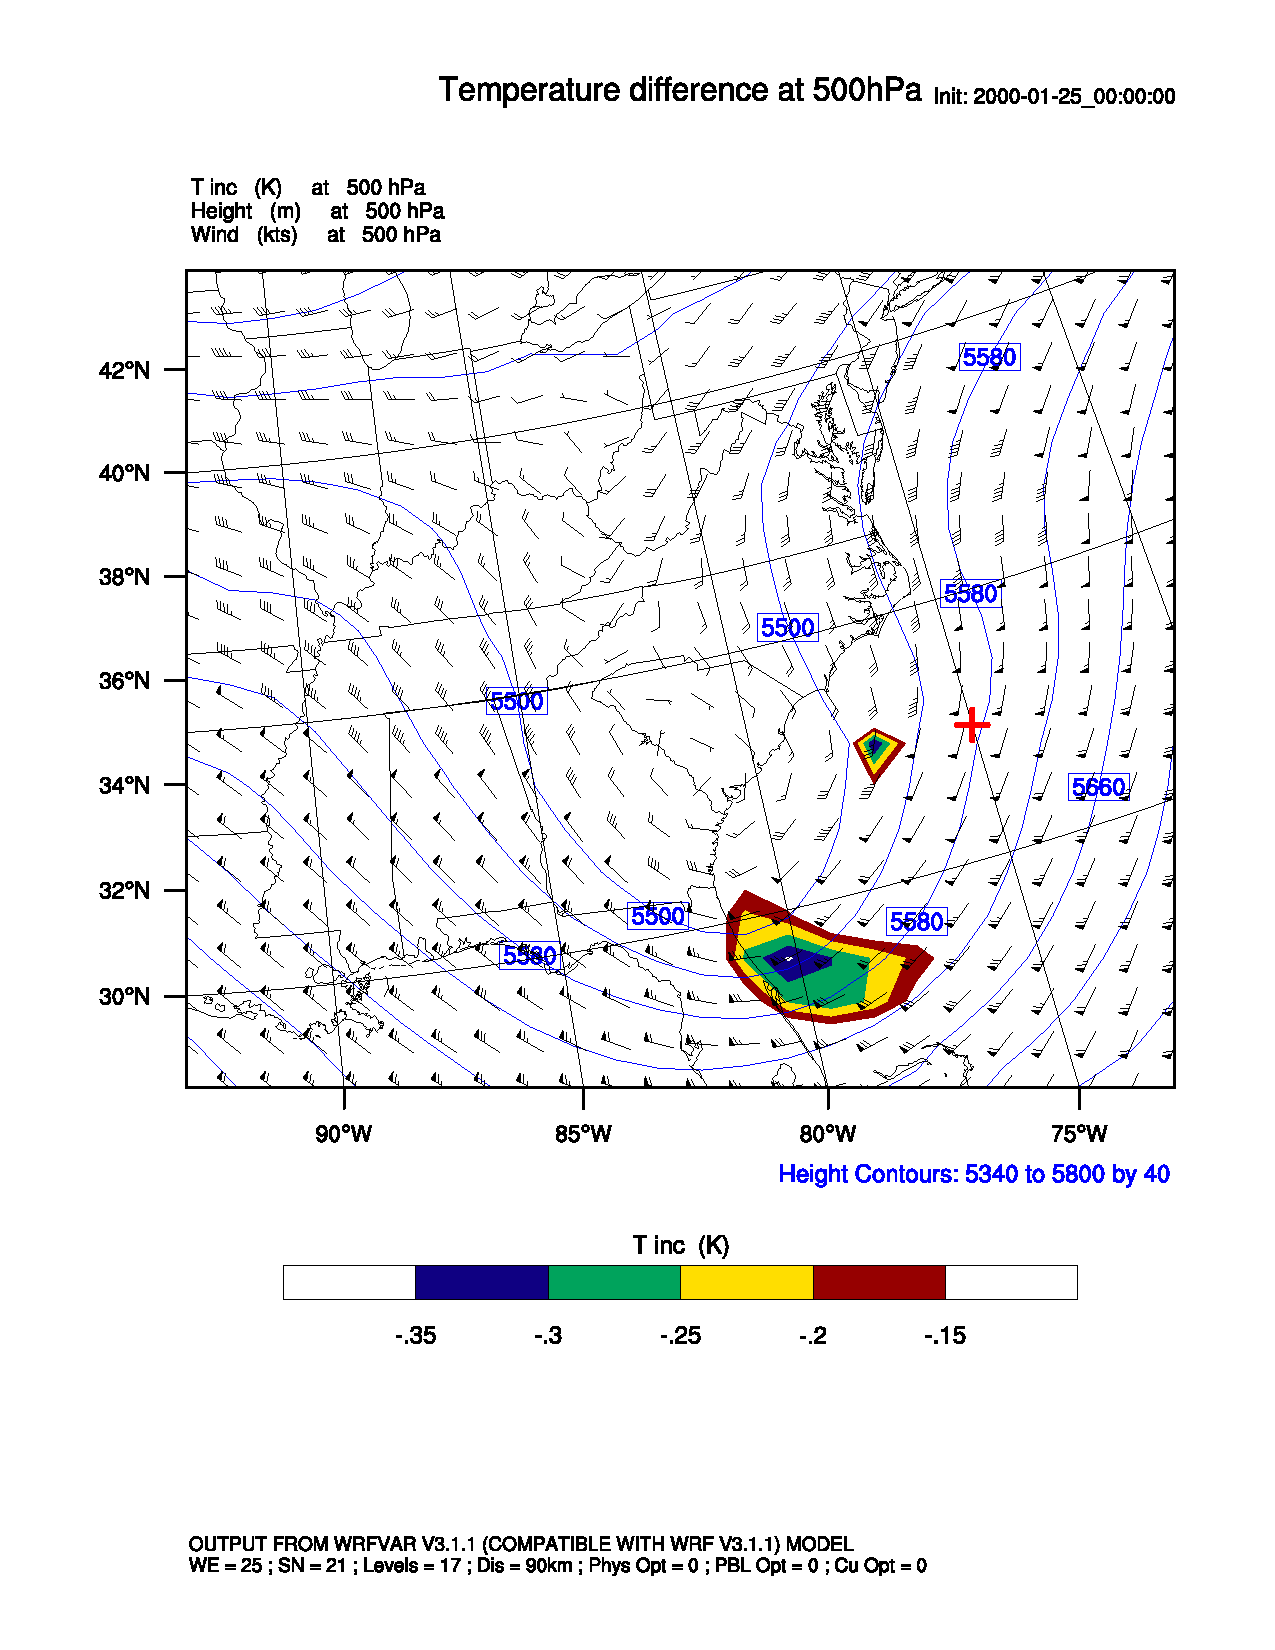
\includegraphics[trim=0 100 0 120, clip=true, width=0.90\textwidth]{figures/center_lbc}
			\caption {with LBC control}
		\end{figure}
	\end{column}
\end{columns}
\end{frame}

%\begin{frame}
%\frametitle{500hPa $\theta$ increments from 0--6 h w/o LBC control}
%\begin{figure} 
%\centering 
%\begin{minipage}[c]{0.3\linewidth} 
%\centering \includegraphics[trim=0 220 0 110, clip=true, width=1.0\textwidth]{figures/center} 
%\end{minipage}% 
%\begin{minipage}[c]{0.8\linewidth} 
%\centering \includegraphics[trim=100 0 60 0, clip=true, angle=90, width=1.0\textwidth]{figures/center_6h} 
%\end{minipage} 
%\end{figure} 
%\end{frame}

\begin{frame}
\frametitle{500hPa $\theta$ increments from 0--6 h w/o LBC control}
\begin{figure} 
\centering 
\centering \includegraphics[trim=40 230 40 110, clip=true, width=0.7\textwidth]{figures/center} 
\end{figure} 
\end{frame}

\begin{frame}
\frametitle{500hPa $\theta$ increments from 0--6 h w/o LBC control}
\begin{figure} 
\centering 
\centering \includegraphics[trim=363 500 66 85, clip=true, angle=90, width=0.7\textwidth]{figures/center_6h} 
\end{figure} 
\end{frame}

\begin{frame}
\frametitle{500hPa $\theta$ increments from 0--6 h w/o LBC control}
\begin{figure} 
\centering 
\centering \includegraphics[trim=363 291 66 295, clip=true, angle=90, width=0.7\textwidth]{figures/center_6h} 
\end{figure} 
\end{frame}

\begin{frame}
\frametitle{500hPa $\theta$ increments from 0--6 h w/o LBC control}
\begin{figure} 
\centering 
\centering \includegraphics[trim=363 82 66 502, clip=true, angle=90, width=0.7\textwidth]{figures/center_6h} 
\end{figure} 
\end{frame}

\begin{frame}
\frametitle{500hPa $\theta$ increments from 0--6 h w/o LBC control}
\begin{figure} 
\centering 
\centering \includegraphics[trim=132 500 300 85, clip=true, angle=90, width=0.7\textwidth]{figures/center_6h} 
\end{figure} 
\end{frame}

\begin{frame}
\frametitle{500hPa $\theta$ increments from 0--6 h w/o LBC control}
\begin{figure} 
\centering 
\centering \includegraphics[trim=132 291 300 293, clip=true, angle=90, width=0.7\textwidth]{figures/center_6h} 
\end{figure} 
\end{frame}

\begin{frame}
\frametitle{500hPa $\theta$ increments from 0--6 h w/o LBC control}
\begin{figure} 
\centering 
\centering \includegraphics[trim=132 82 300 502, clip=true, angle=90, width=0.7\textwidth]{figures/center_6h} 
\end{figure} 
\end{frame}

%\begin{frame}
%\frametitle{500hPa $\theta$ increments from 0--6 h with LBC control}
%\animate<2-4>
%\begin{figure} 
%\centering 
%\begin{minipage}[c]{0.3\linewidth} 
%\centering 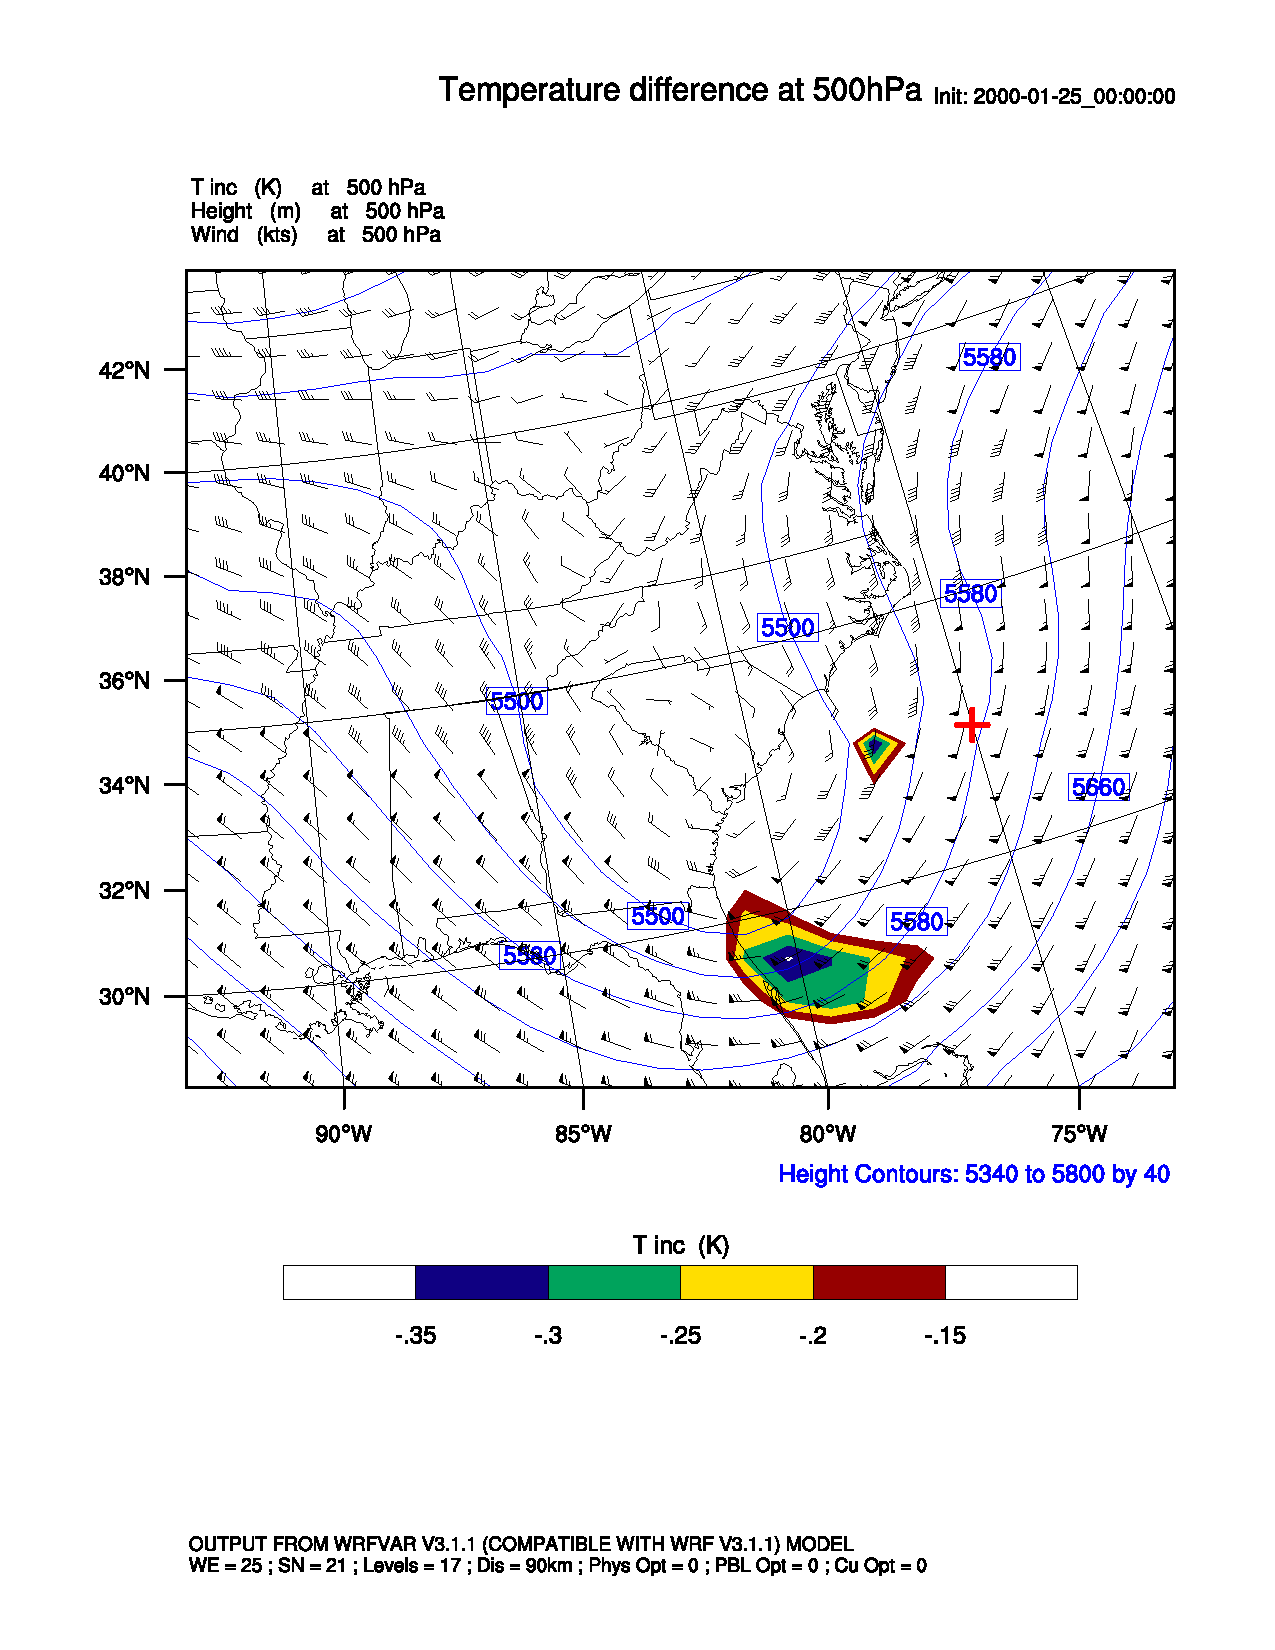
\includegraphics[trim=0 220 0 110, clip=true, width=1.0\textwidth]{figures/center_lbc} 
%\end{minipage}% 
%\begin{minipage}[c]{0.8\linewidth} 
%\centering 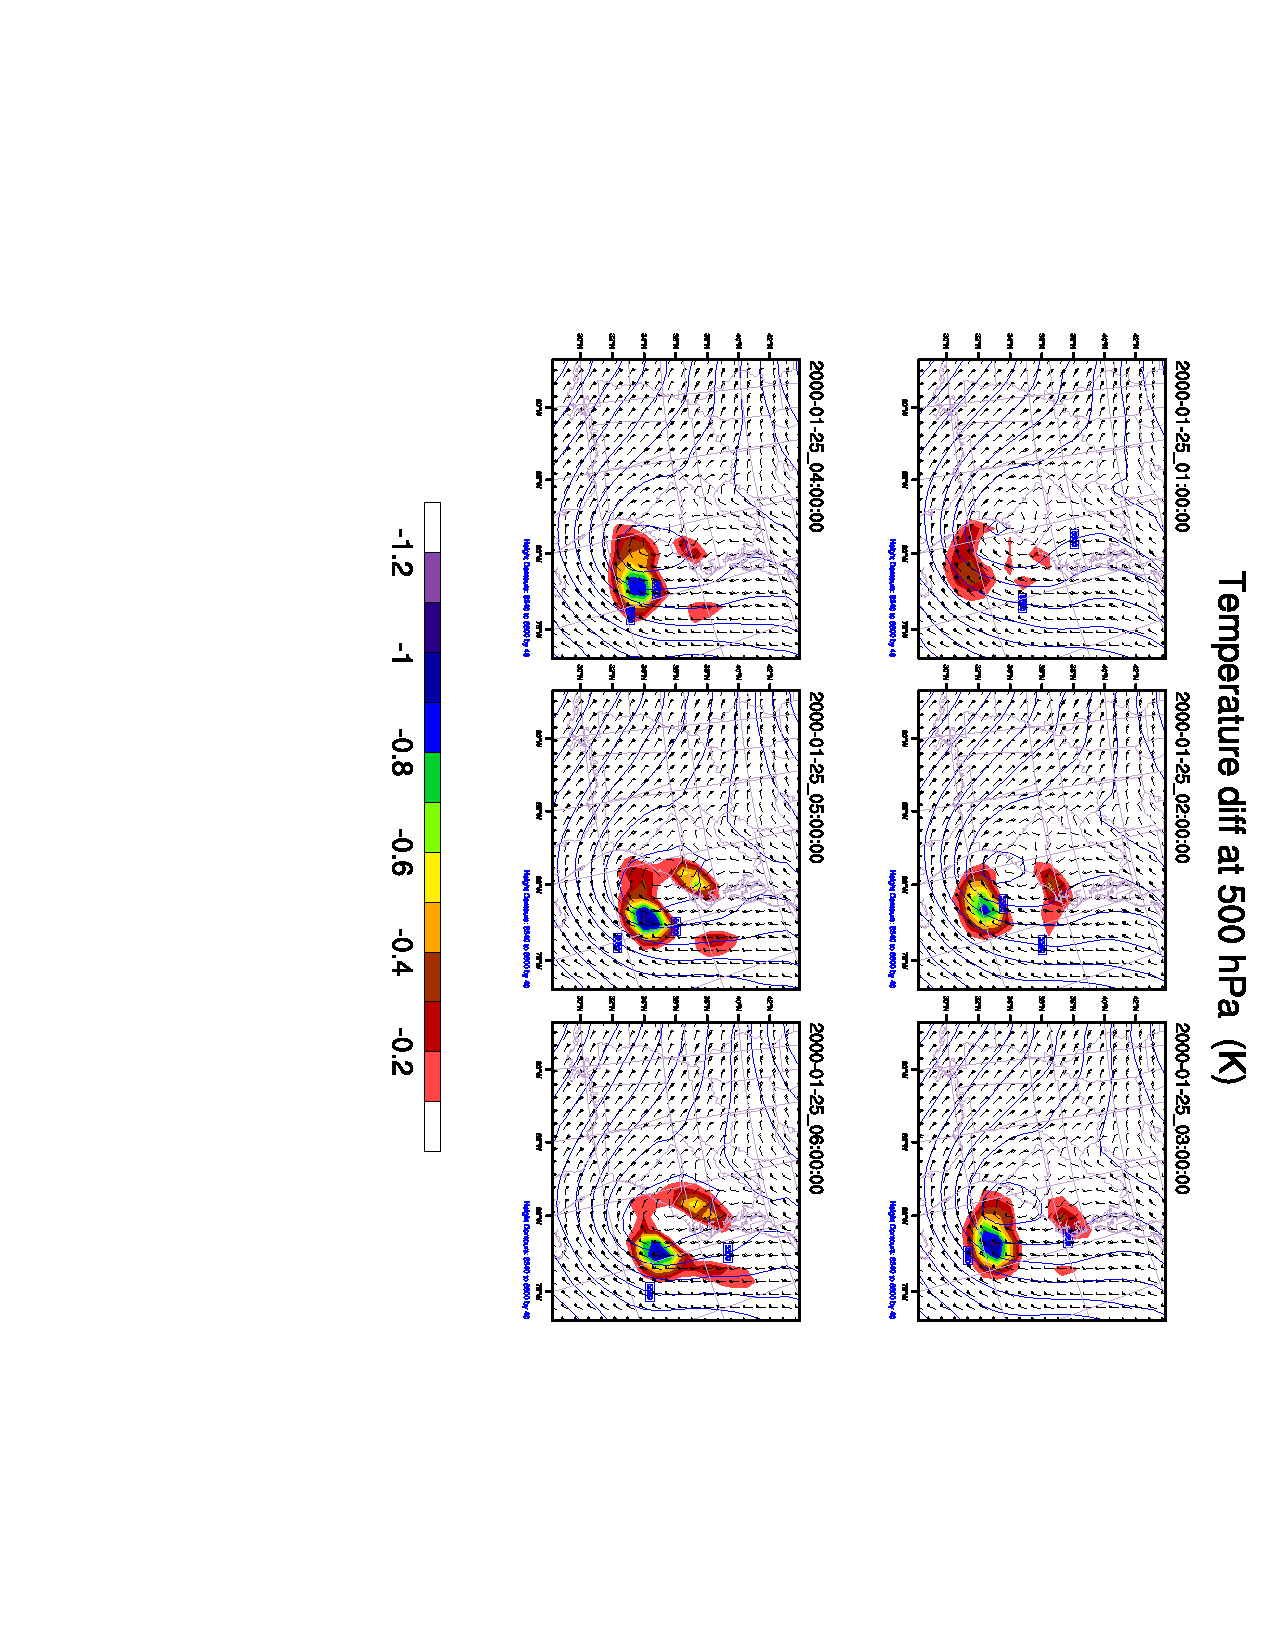
\includegraphics[trim=100 0 60 0, clip=true, angle=90, width=1.0\textwidth]{figures/center_lbc_6h} 
%\end{minipage} 
%\end{figure} 
%\end{frame}

\begin{frame}
\frametitle{500hPa $\theta$ increments from 0--6 h with LBC control}
\begin{figure} 
\centering 
\centering 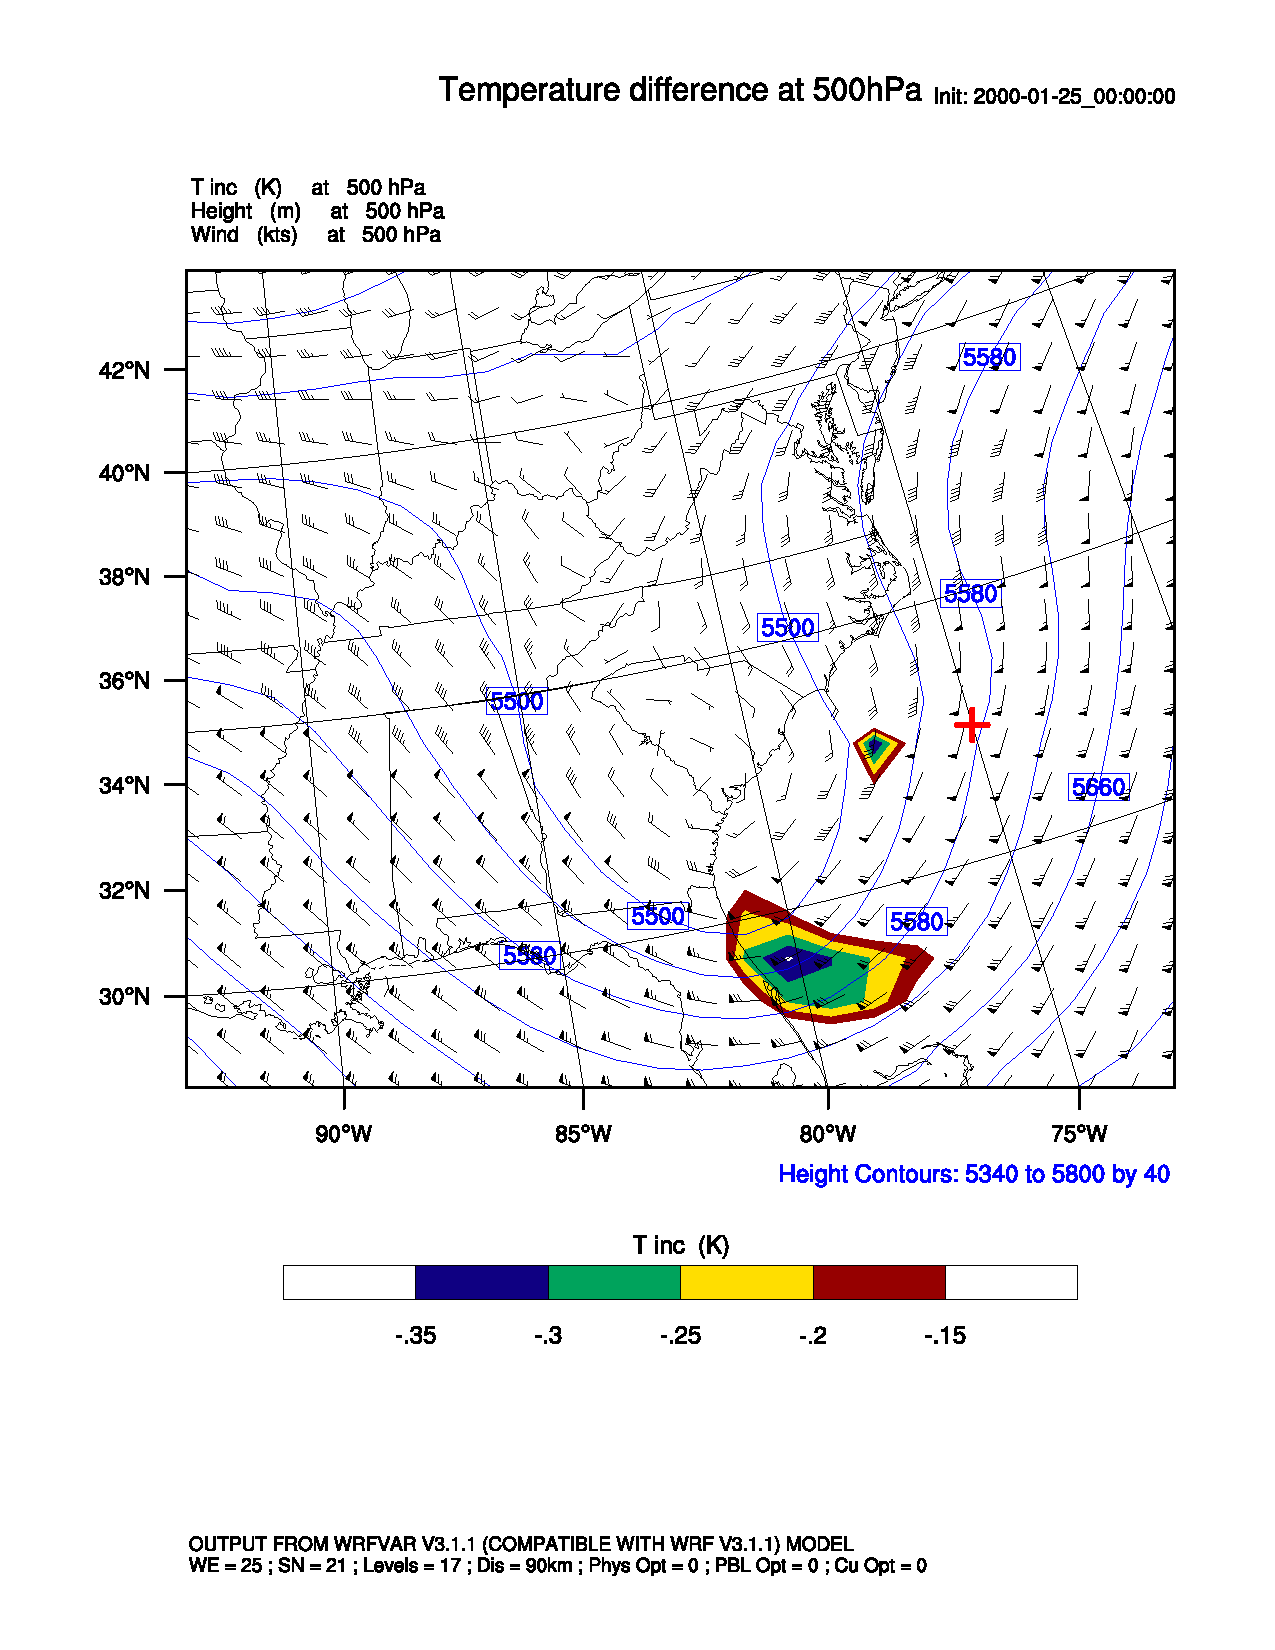
\includegraphics[trim=40 230 40 110, clip=true, width=0.7\textwidth]{figures/center_lbc} 
\end{figure} 
\end{frame}

\begin{frame}
\frametitle{500hPa $\theta$ increments from 0--6 h with LBC control}
\begin{figure} 
\centering 
\centering 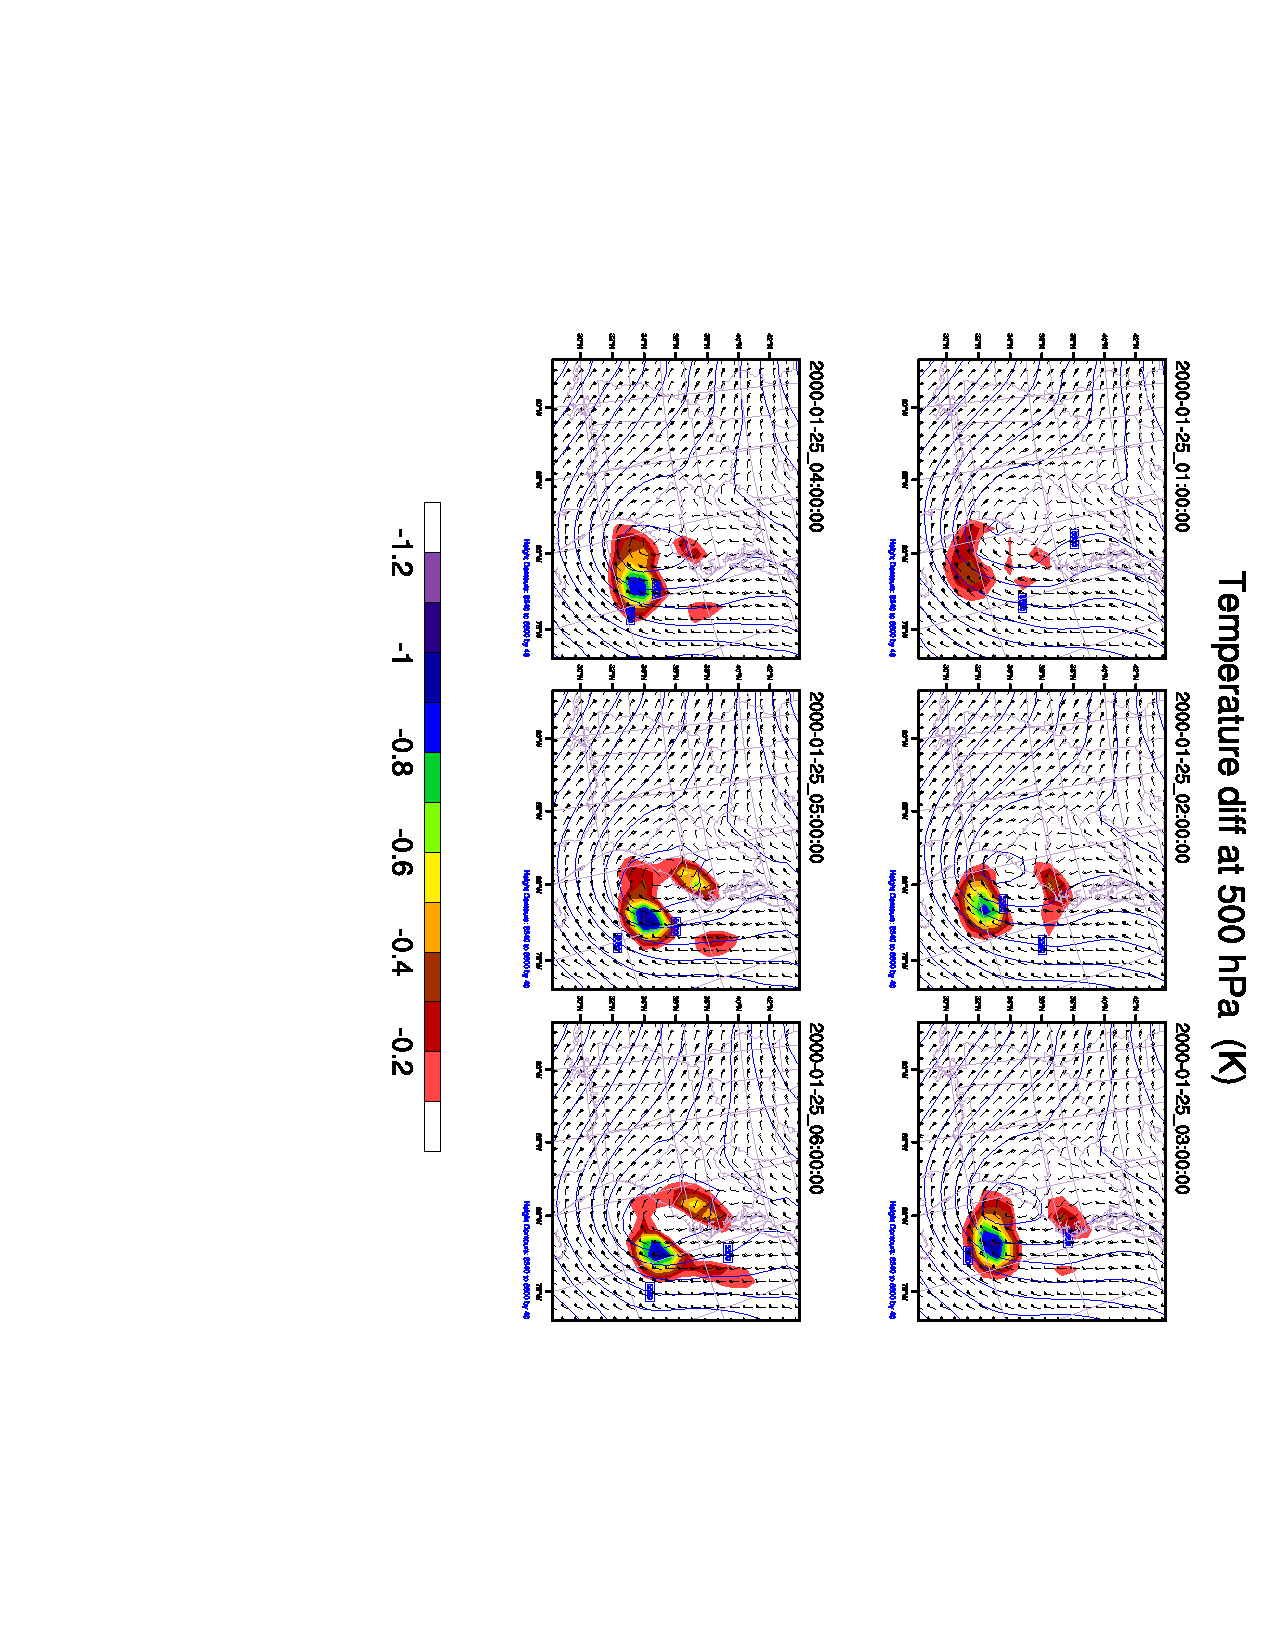
\includegraphics[trim=363 500 66 85, clip=true, angle=90, width=0.7\textwidth]{figures/center_lbc_6h} 
\end{figure} 
\end{frame}

\begin{frame}
\frametitle{500hPa $\theta$ increments from 0--6 h with LBC control}
\begin{figure} 
\centering 
\centering 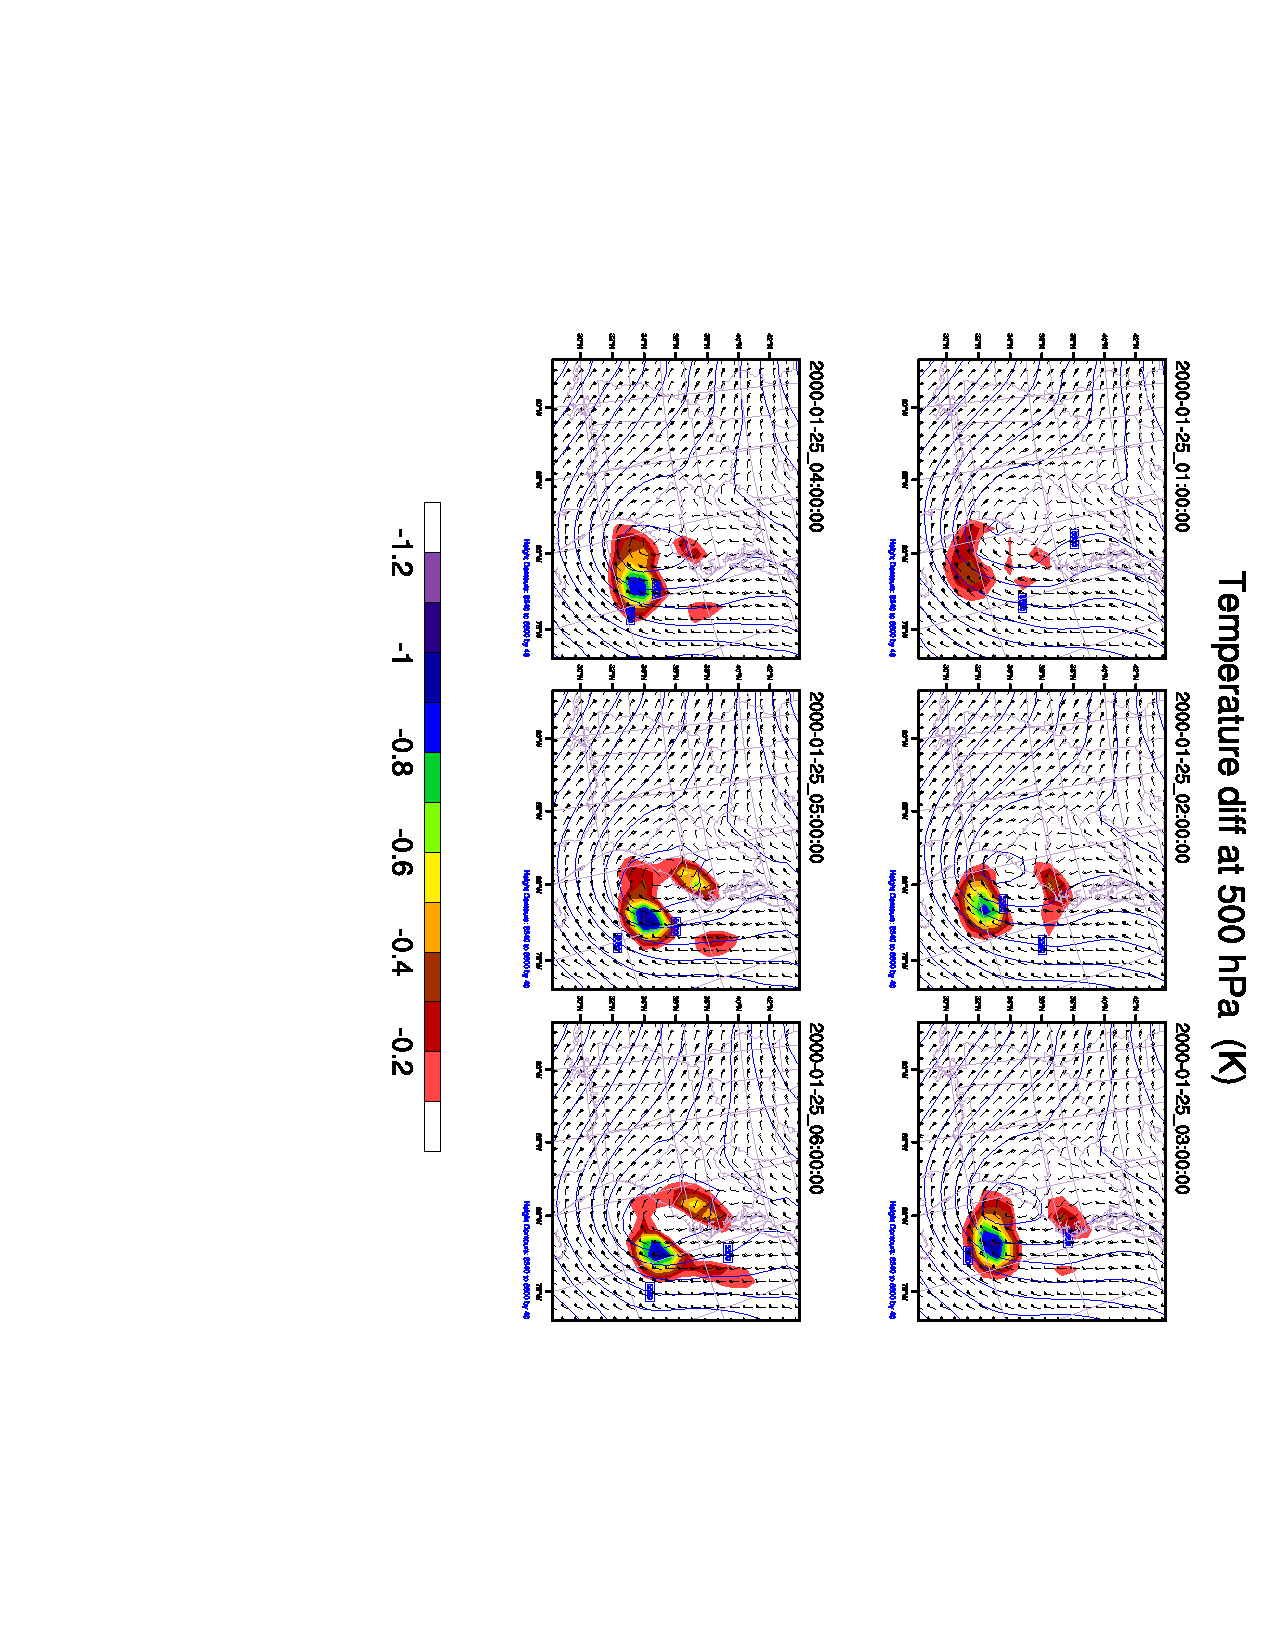
\includegraphics[trim=363 291 66 295, clip=true, angle=90, width=0.7\textwidth]{figures/center_lbc_6h} 
\end{figure} 
\end{frame}

\begin{frame}
\frametitle{500hPa $\theta$ increments from 0--6 h with LBC control}
\begin{figure} 
\centering 
\centering 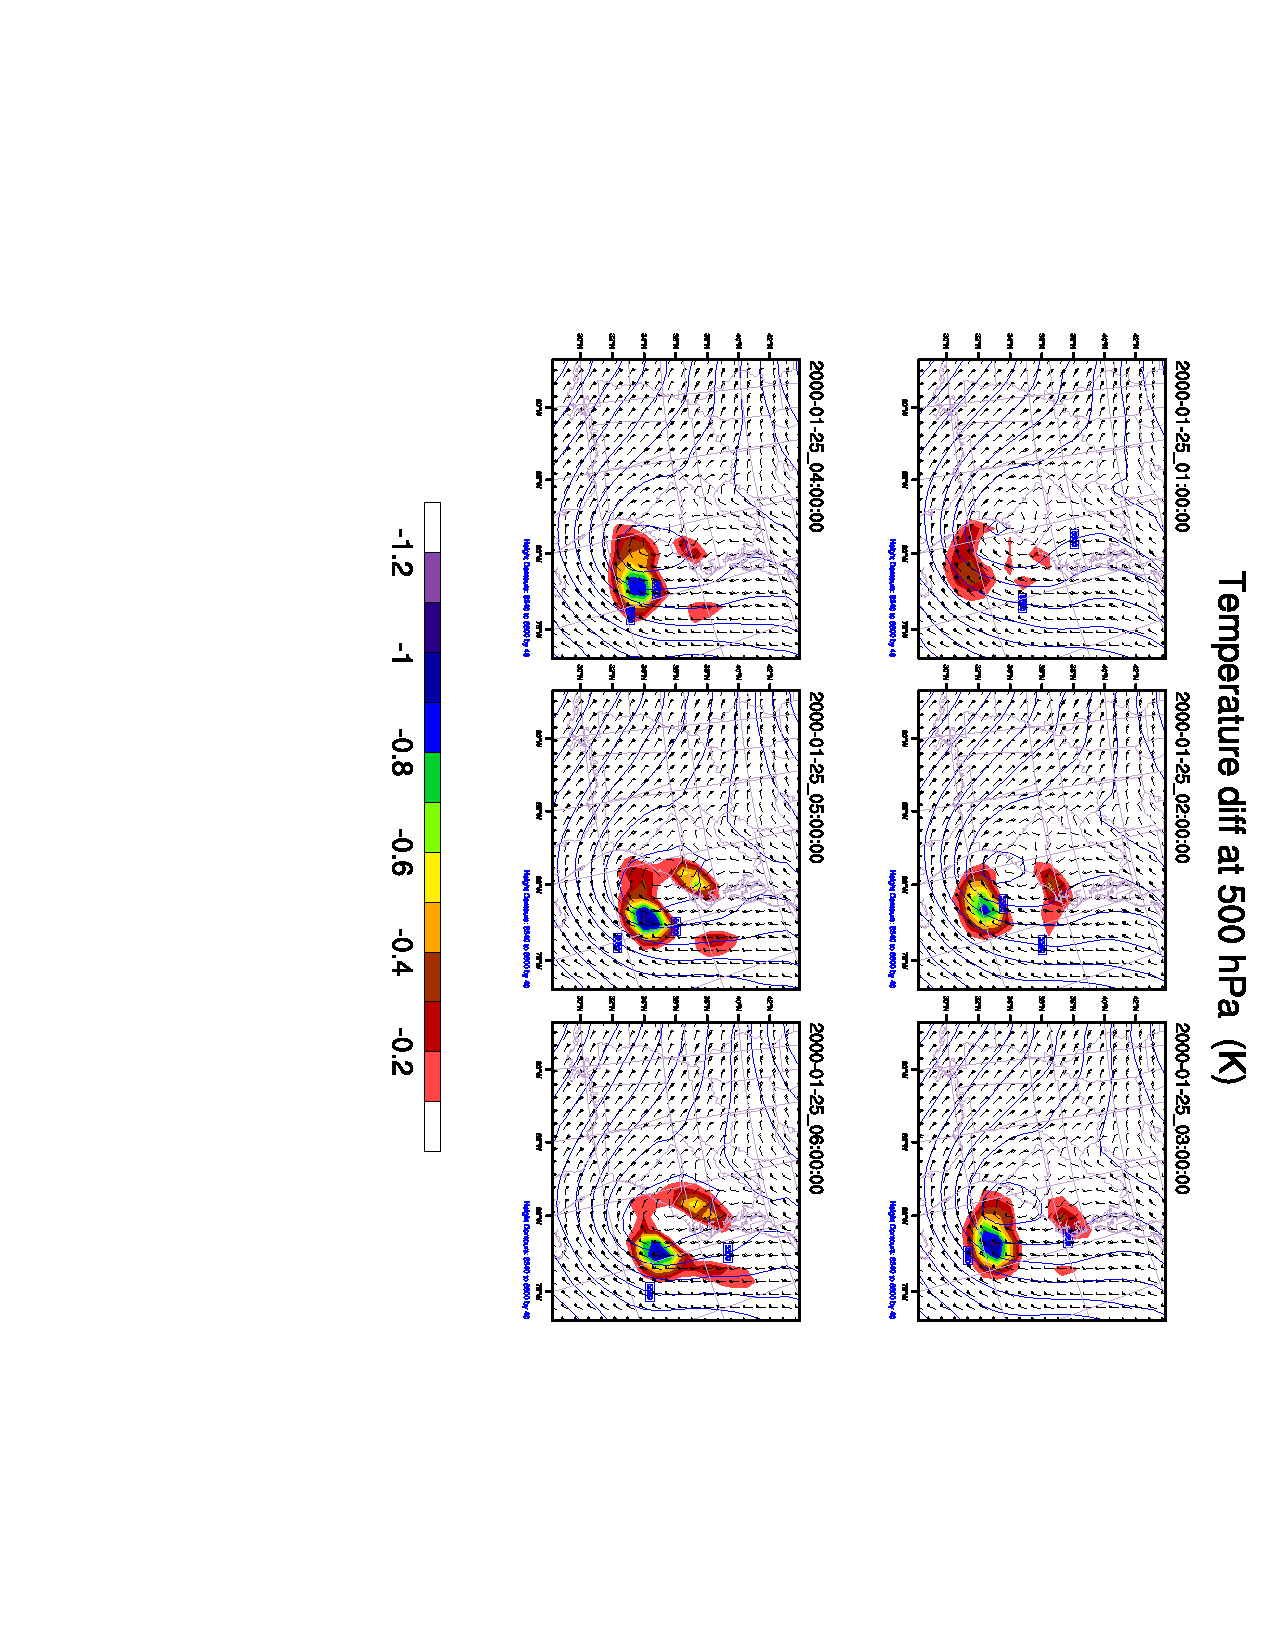
\includegraphics[trim=363 82 66 502, clip=true, angle=90, width=0.7\textwidth]{figures/center_lbc_6h} 
\end{figure} 
\end{frame}

\begin{frame}
\frametitle{500hPa $\theta$ increments from 0--6 h with LBC control}
\begin{figure} 
\centering 
\centering 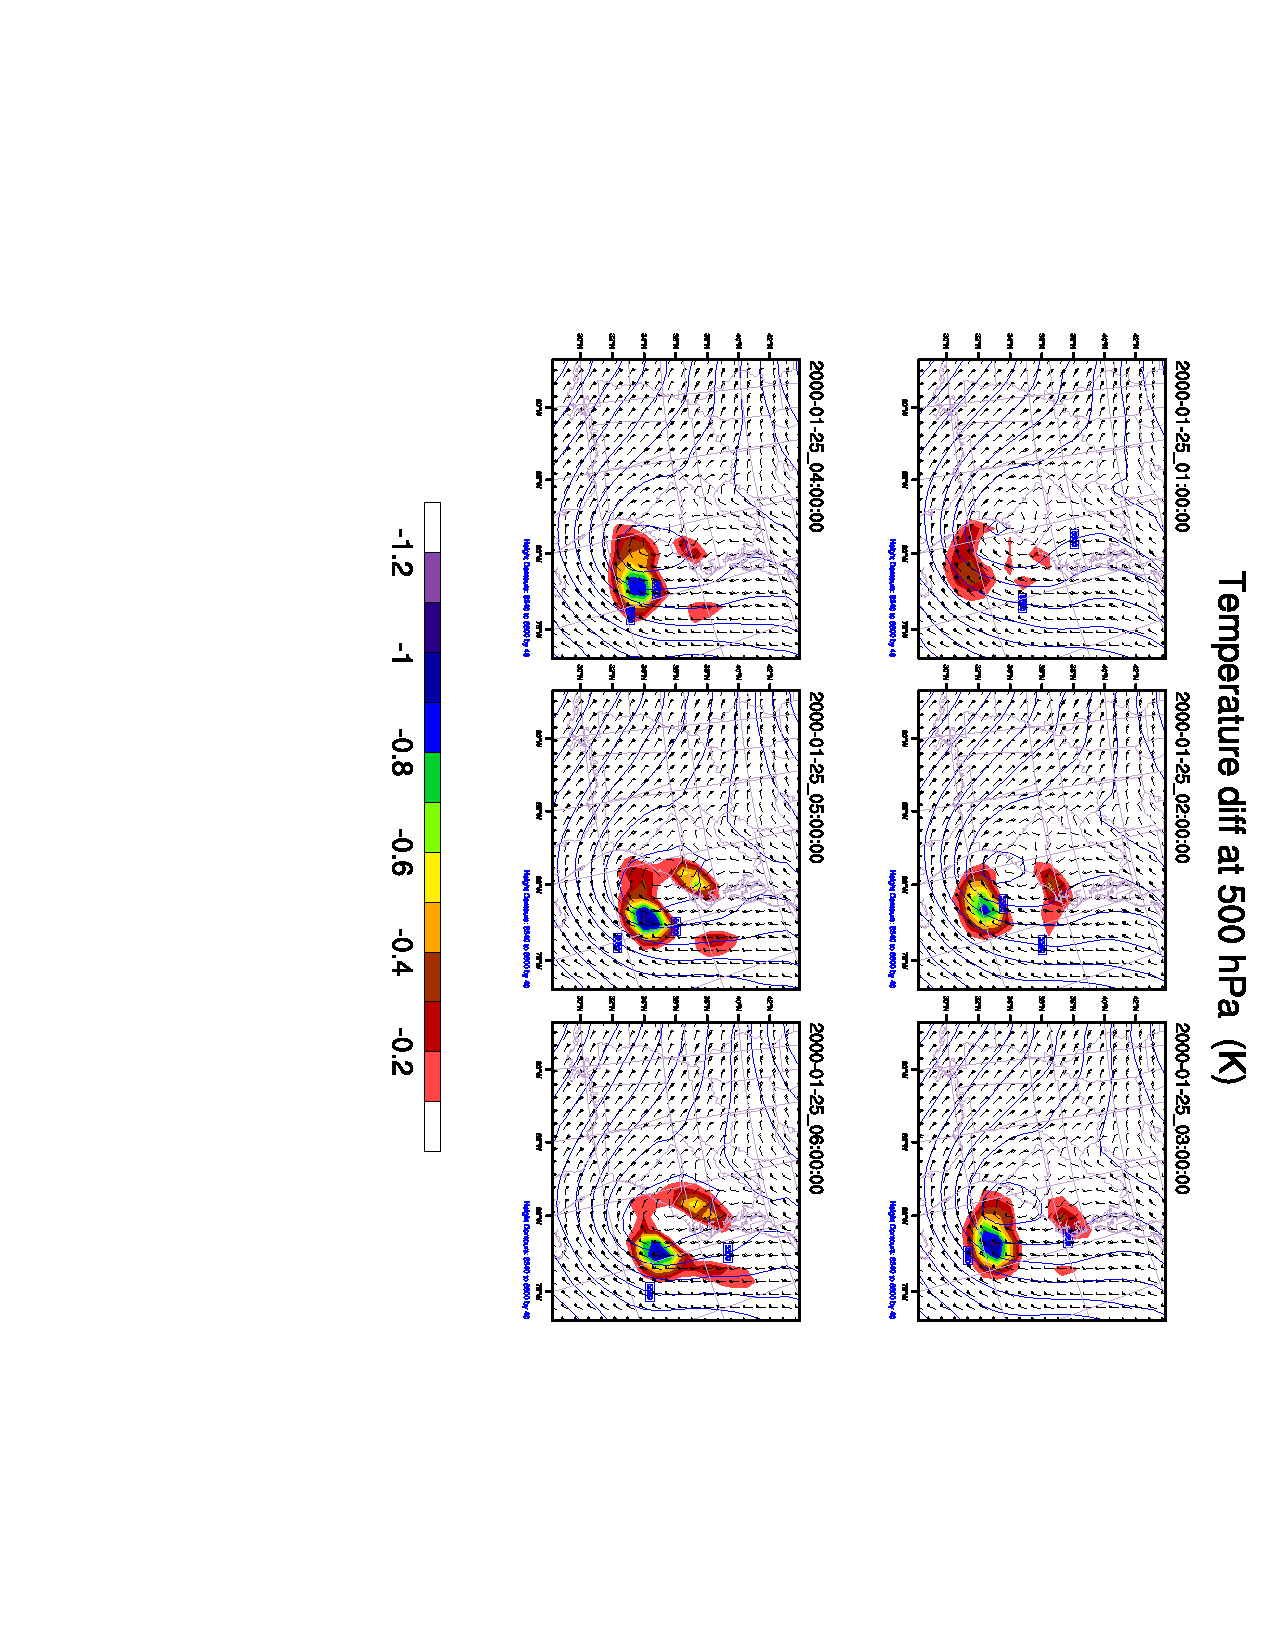
\includegraphics[trim=132 500 300 85, clip=true, angle=90, width=0.7\textwidth]{figures/center_lbc_6h} 
\end{figure} 
\end{frame}

\begin{frame}
\frametitle{500hPa $\theta$ increments from 0--6 h with LBC control}
\begin{figure} 
\centering 
\centering 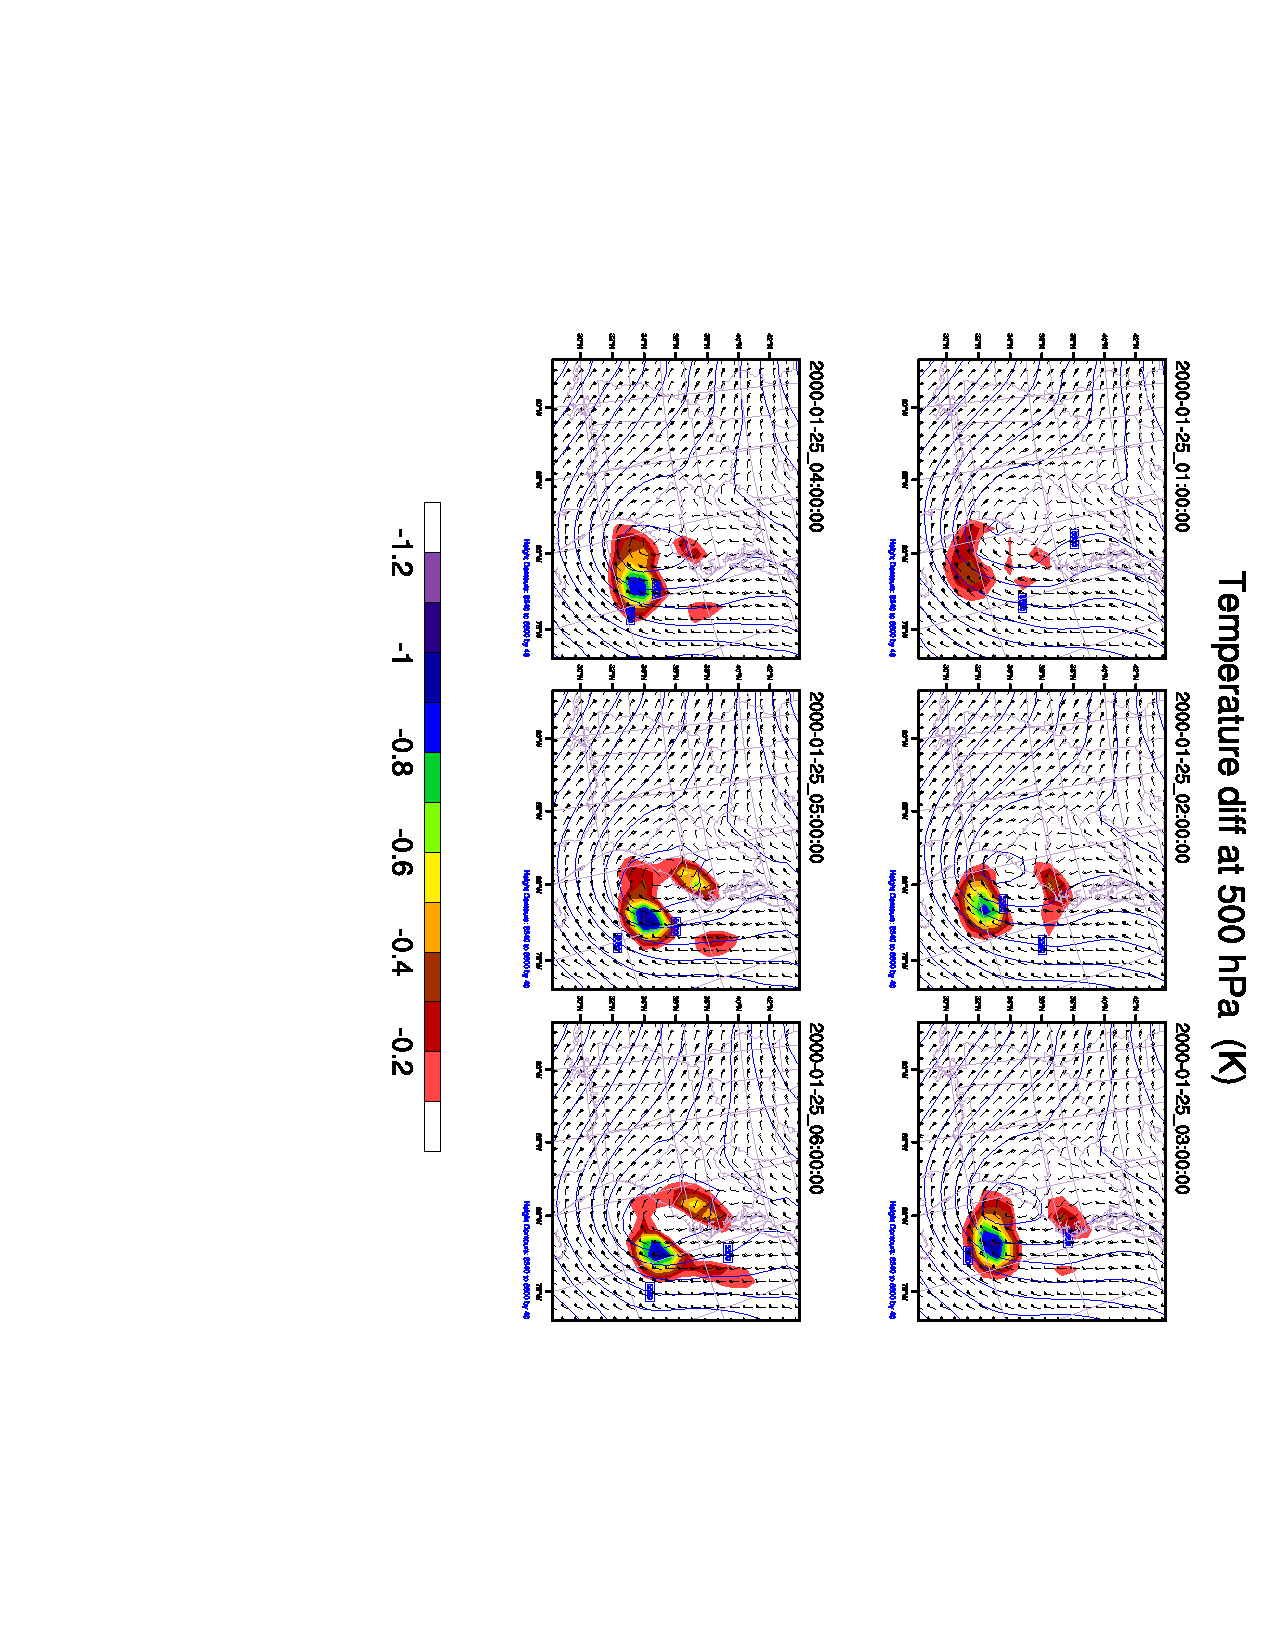
\includegraphics[trim=132 291 300 293, clip=true, angle=90, width=0.7\textwidth]{figures/center_lbc_6h} 
\end{figure} 
\end{frame}

\begin{frame}
\frametitle{500hPa $\theta$ increments from 0--6 h with LBC control}
\begin{figure} 
\centering 
\centering 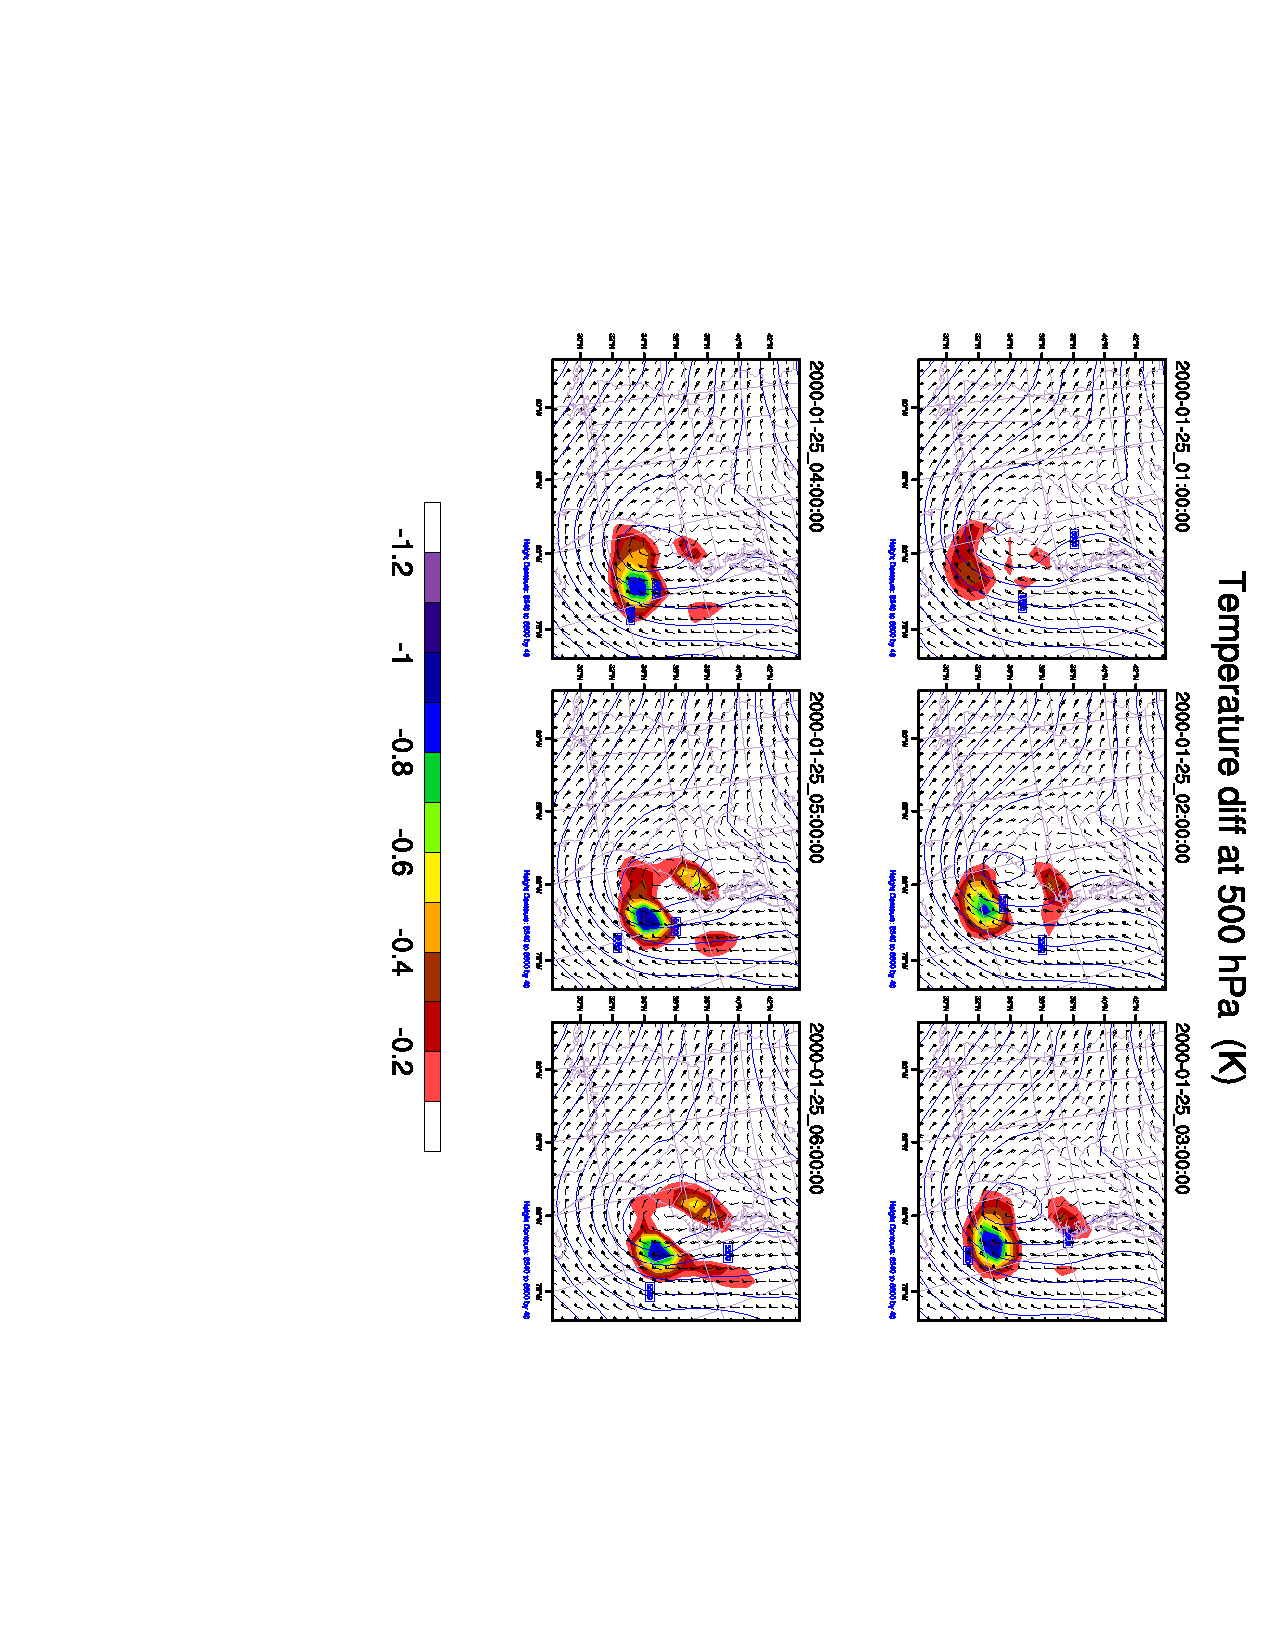
\includegraphics[trim=132 82 300 502, clip=true, angle=90, width=0.7\textwidth]{figures/center_lbc_6h} 
\end{figure} 
\end{frame}

\begin{frame}
\frametitle{Remark}
\begin{itemize}
\item The Final $J_{lbc}$ is increased from 0 to 0.01 \pause
\vspace{2mm}
%\item LBC control has some impact on the initial $\theta$ perturbation since it close to the boundary relaxation zone \pause
% Compared the figures w/ and w/o LBC control, the perturbation evolutions are almost the same, which implies that
\item  The LBC control doesn't change the minimization too much if the observation is far away from lateral boundary and out of the reach of the LBC influence during the assimilation window
\end{itemize}
\end{frame}

\subsection{Exp-2: A 6 h observation close to boundary ($\Delta T= 2K$)}

\begin{frame}
\frametitle{500hPa $\theta$ analysis increments at 0 h}
$\color{red}\textbf{+}$ is the location of the observation at 6h
\begin{columns}[t]
	\begin{column}{6cm}
		\begin{figure}
			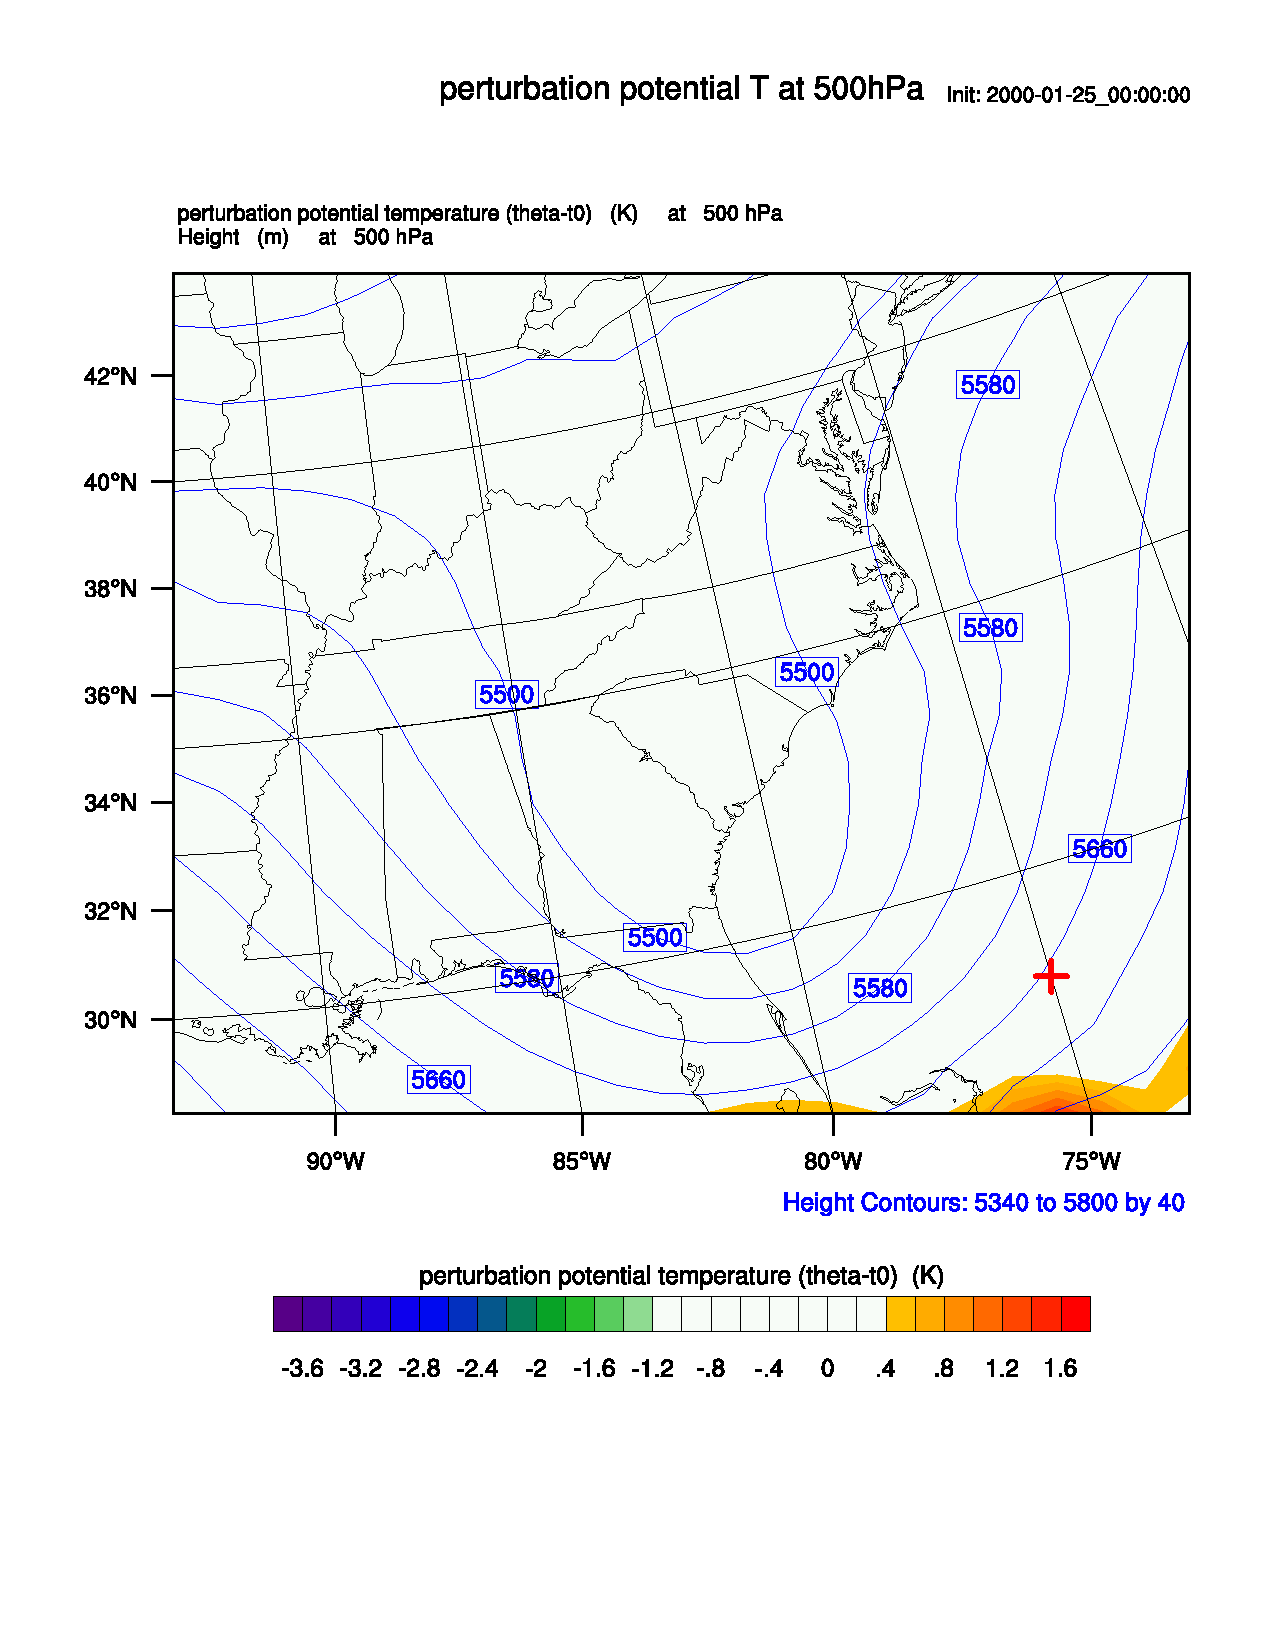
\includegraphics[trim=0 100 0 120, clip=true, width=0.90\textwidth]{figures/boundary}
			\caption {w/o LBC control}
		\end{figure}
	\end{column}
	\begin{column}{6cm}
		\begin{figure}
			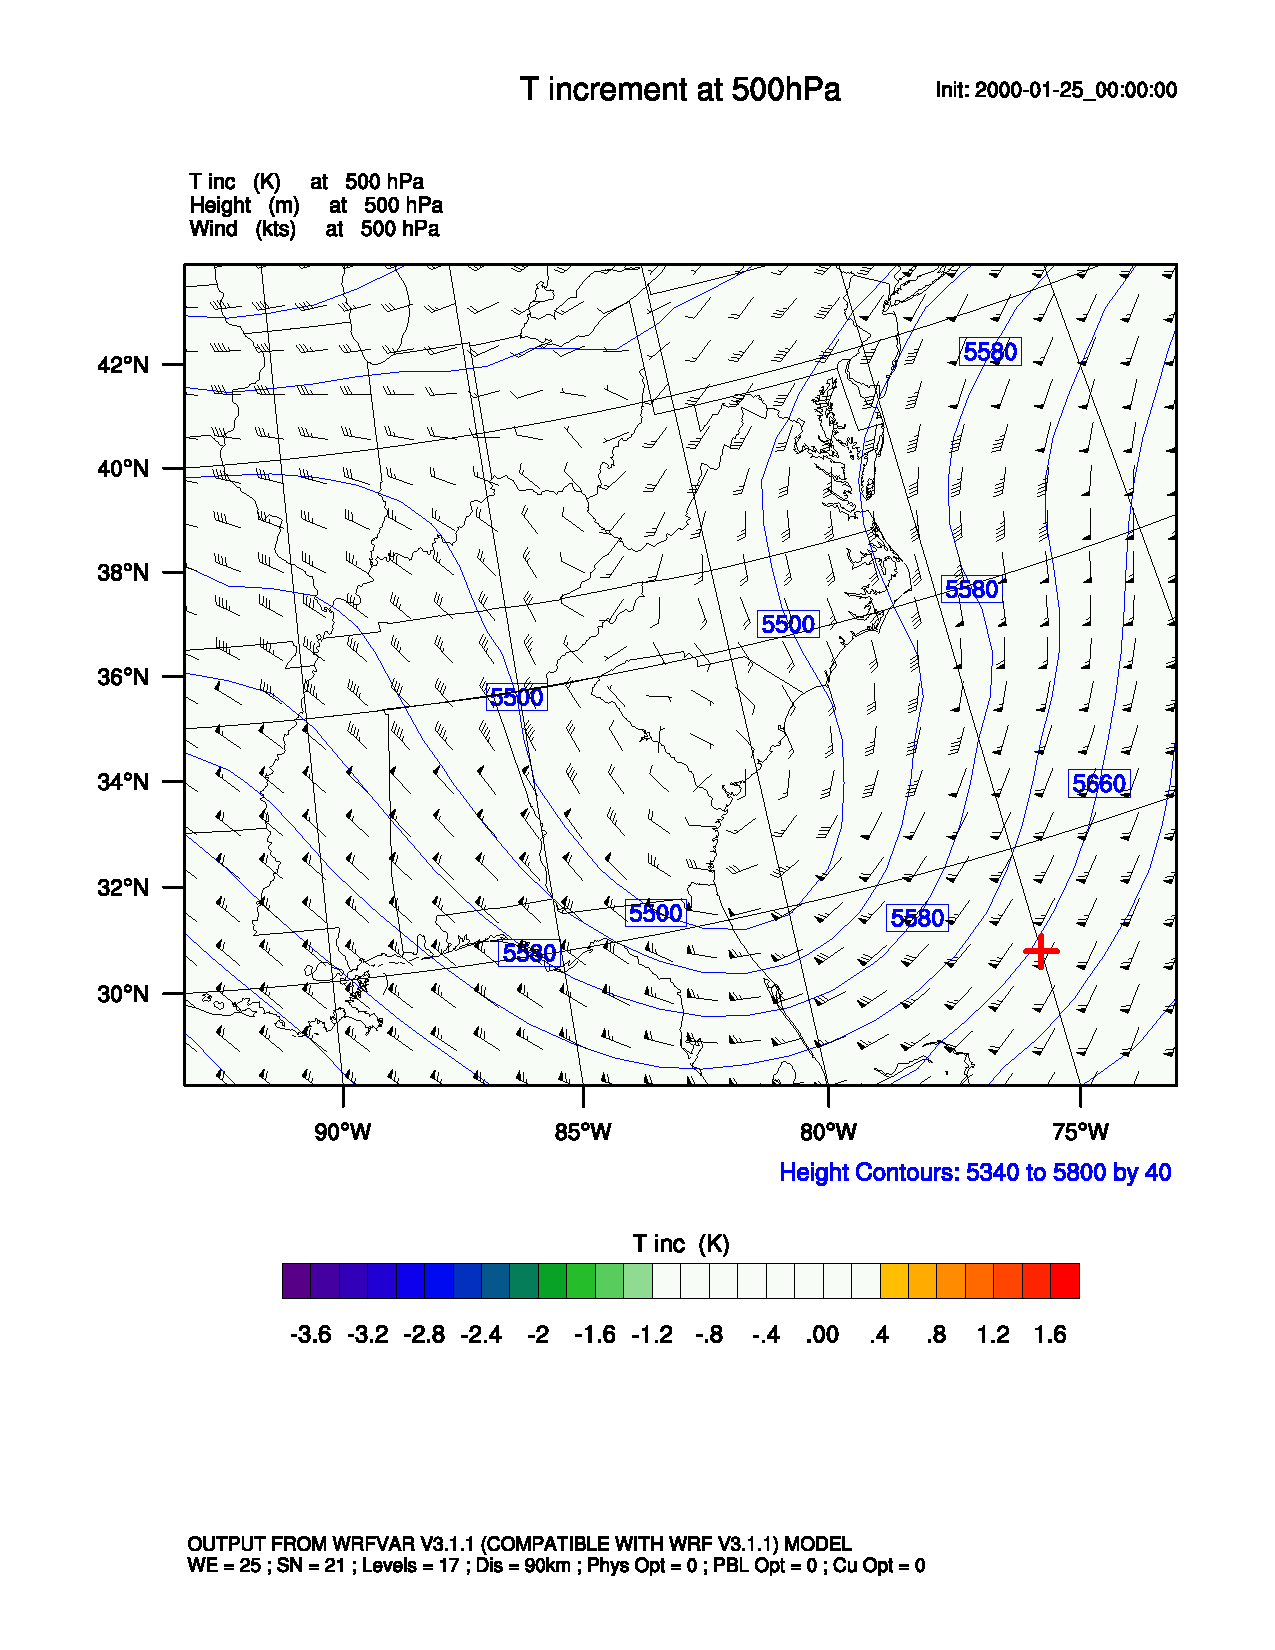
\includegraphics[trim=0 100 0 120, clip=true, width=0.90\textwidth]{figures/boundary_lbc}
			\caption {with LBC control}
		\end{figure}
	\end{column}
\end{columns}
\end{frame}

%\begin{frame}
%\frametitle{500hPa $\theta$ increments 0--6 h w/o LBC control}
%\begin{figure} 
%\centering 
%\begin{minipage}[c]{0.3\linewidth} 
%\centering 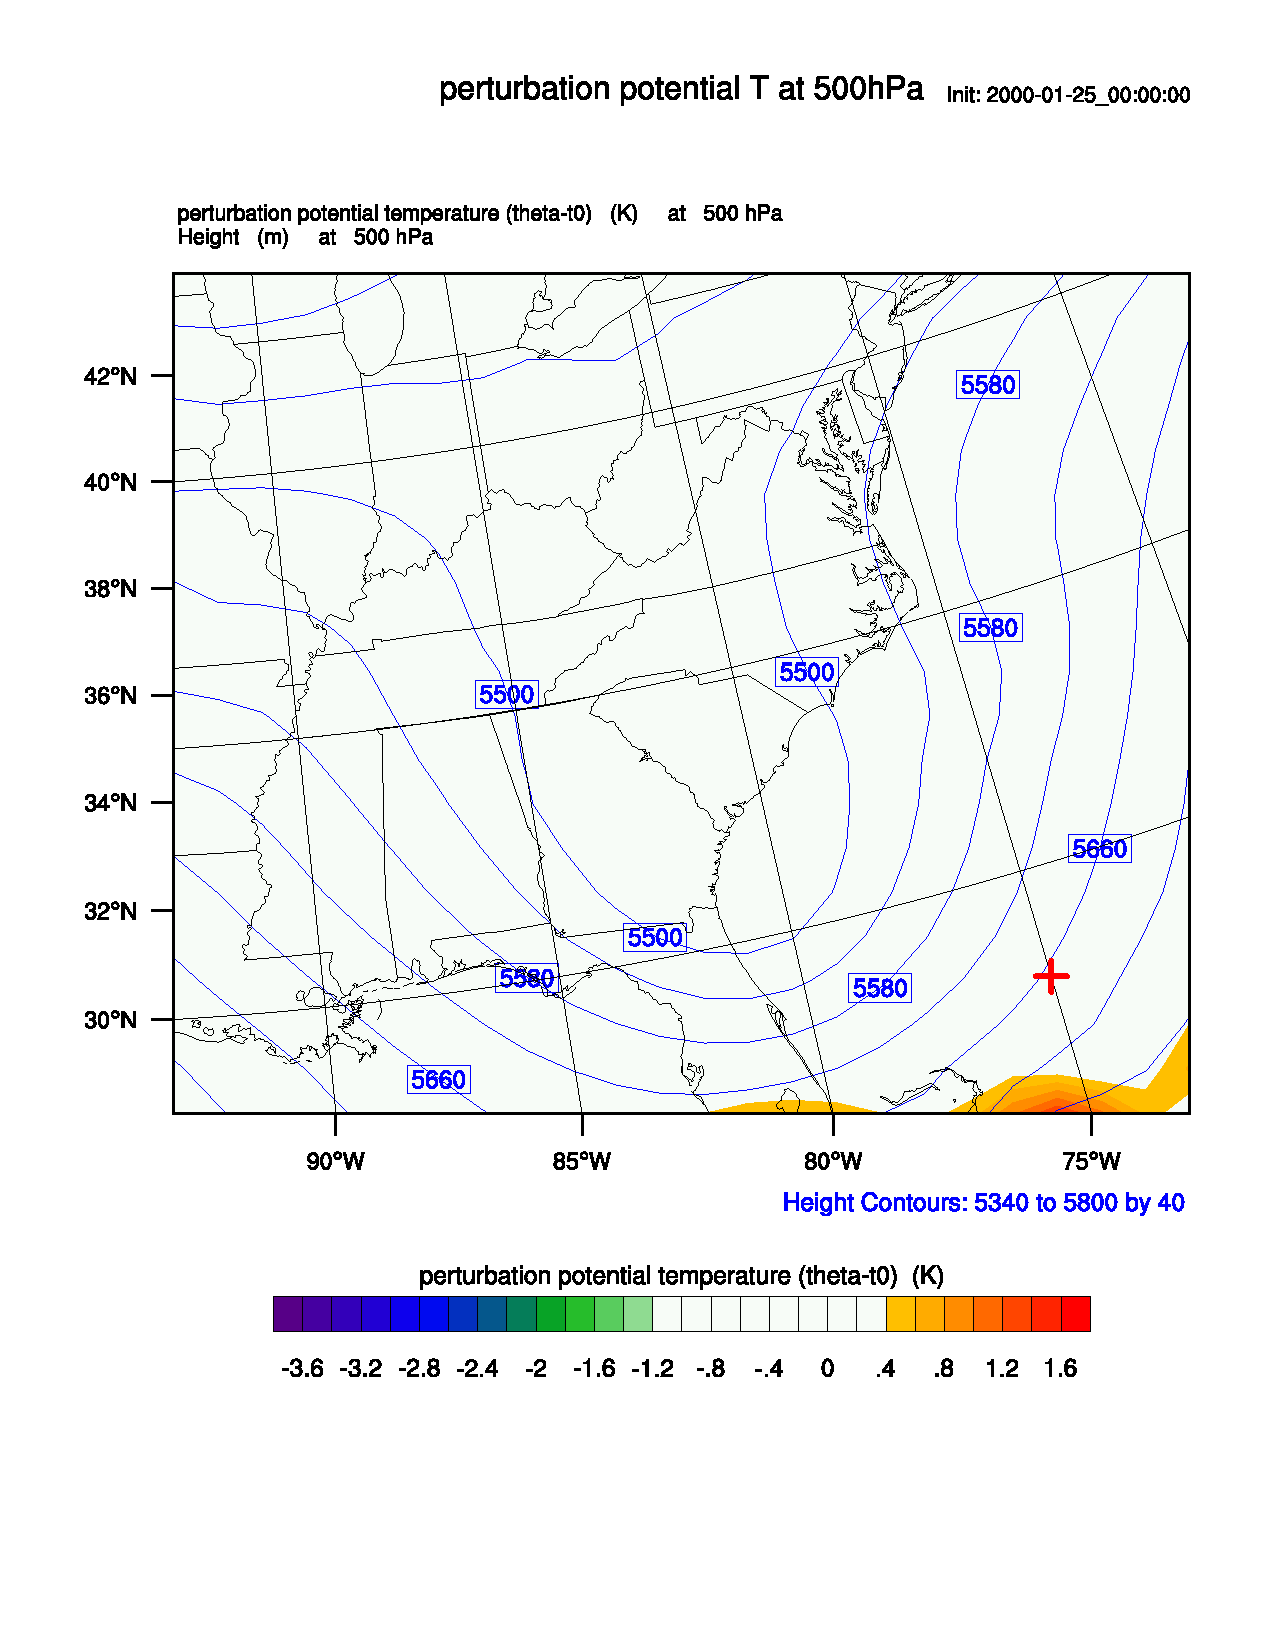
\includegraphics[trim=0 220 0 110, clip=true, width=1.0\textwidth]{figures/boundary} 
%\end{minipage}% 
%\begin{minipage}[c]{0.8\linewidth} 
%\centering 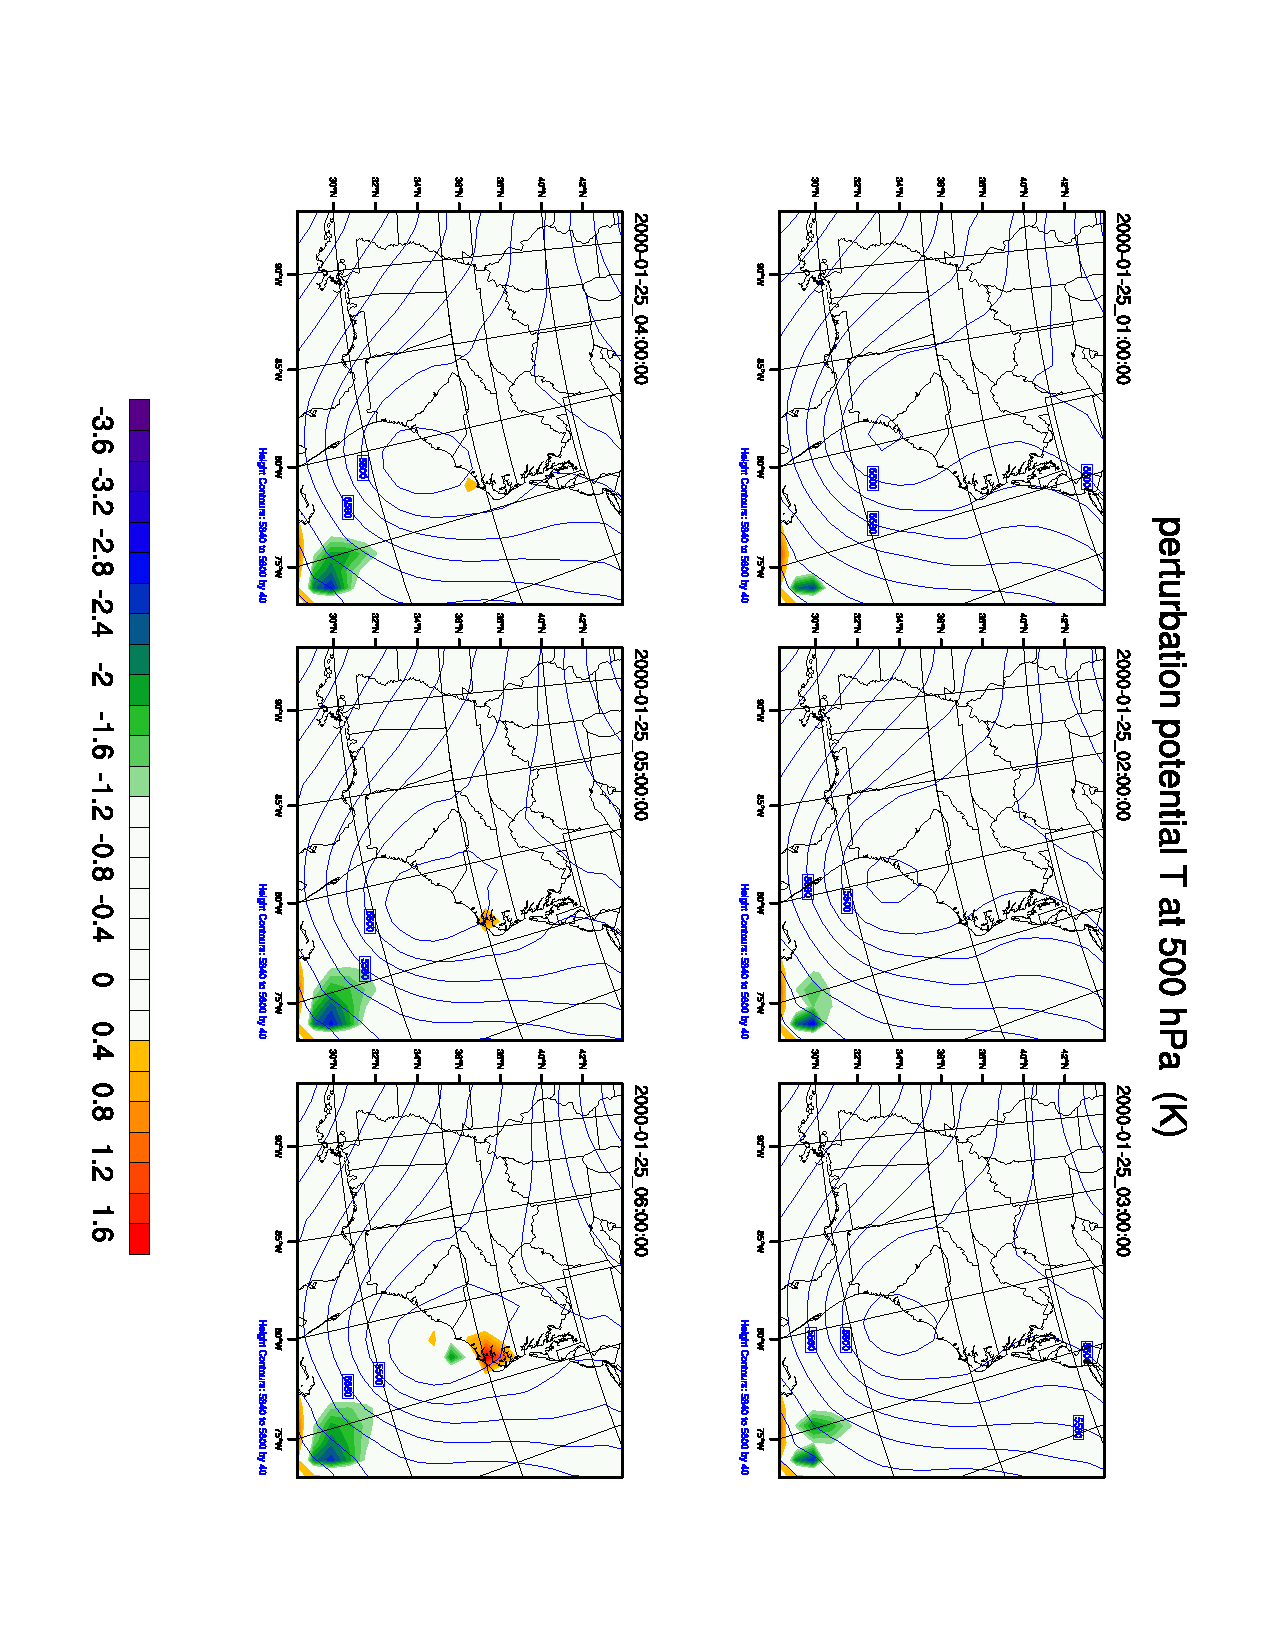
\includegraphics[trim=100 0 60 0, clip=true, angle=90, width=1.0\textwidth]{figures/boundary_6h} 
%\end{minipage} 
%\end{figure} 
%\end{frame}

\begin{frame}
\frametitle{500hPa $\theta$ increments from 0--6 h w/o LBC control}
\begin{figure} 
\centering 
\centering 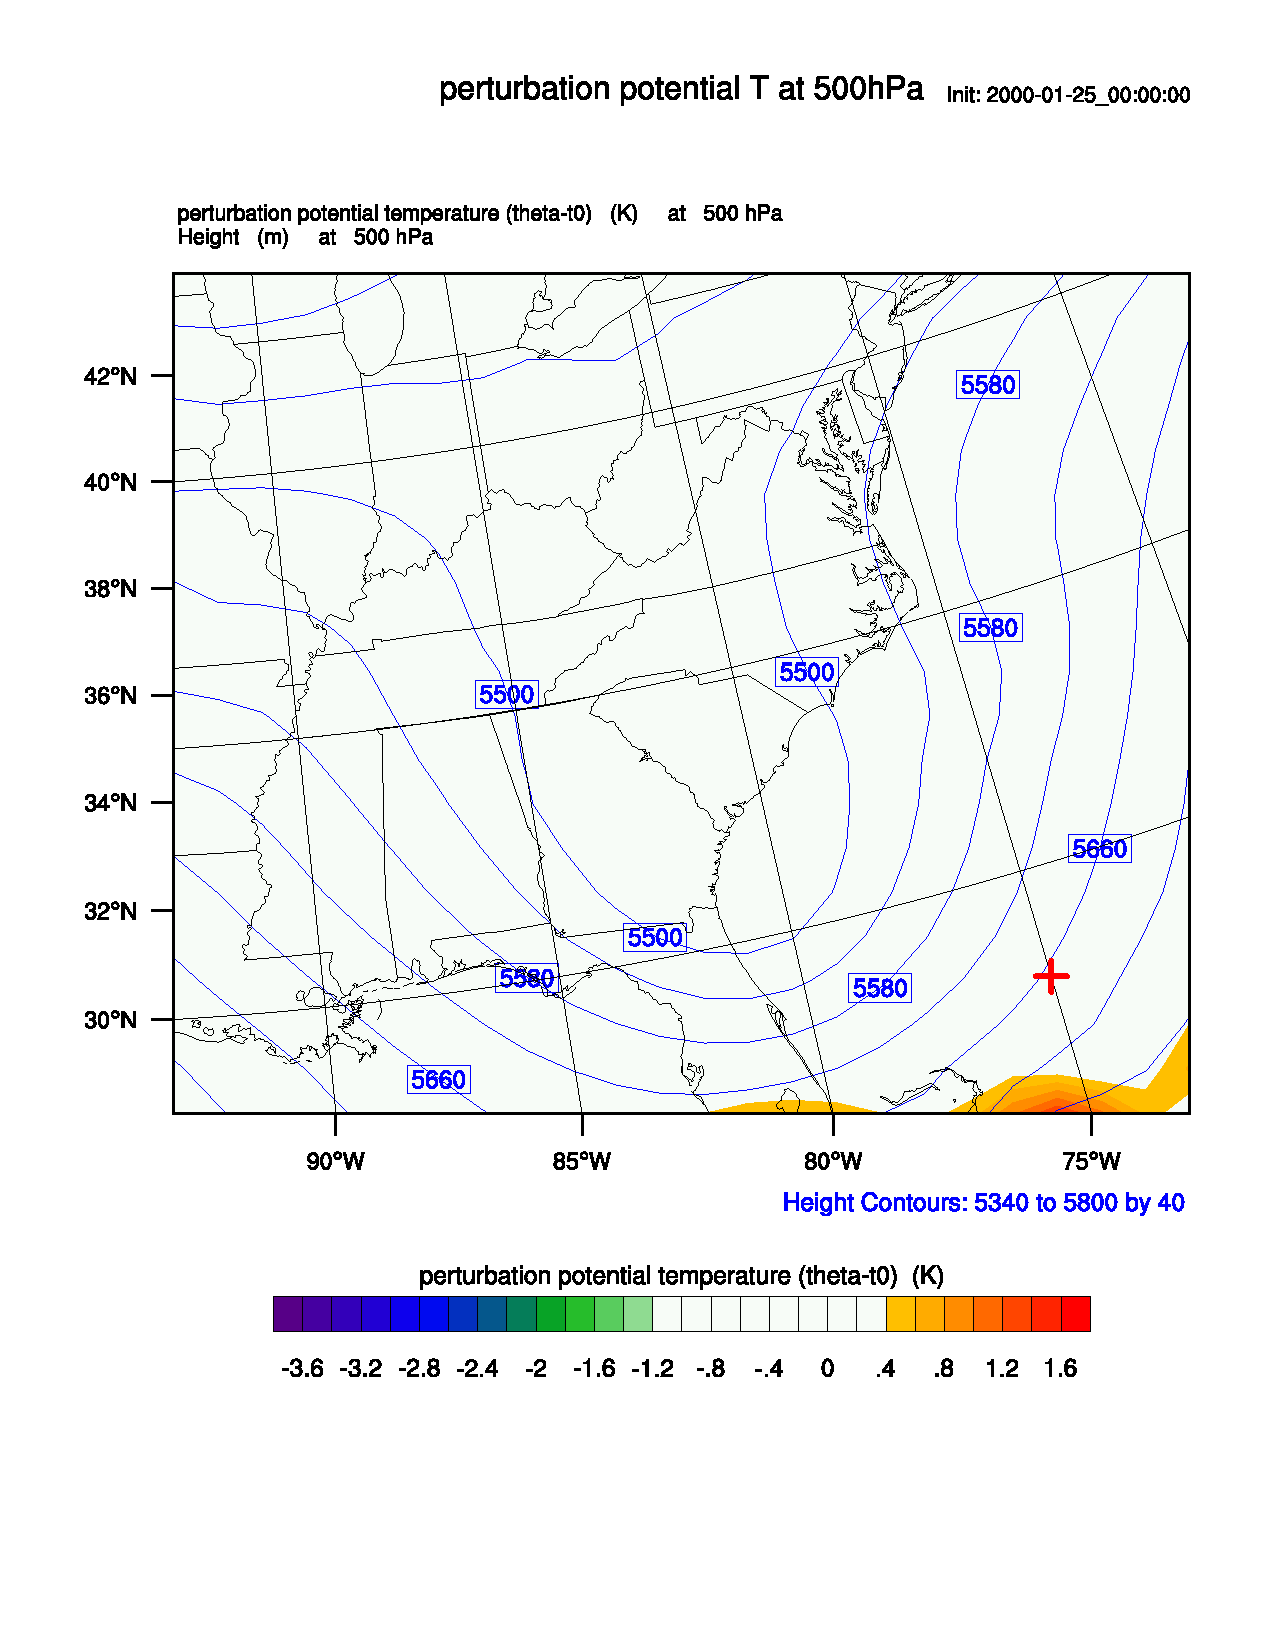
\includegraphics[trim=40 230 40 110, clip=true, width=0.7\textwidth]{figures/boundary} 
\end{figure} 
\end{frame}

\begin{frame}
\frametitle{500hPa $\theta$ increments from 0--6 h w/o LBC control}
\begin{figure} 
\centering 
\centering 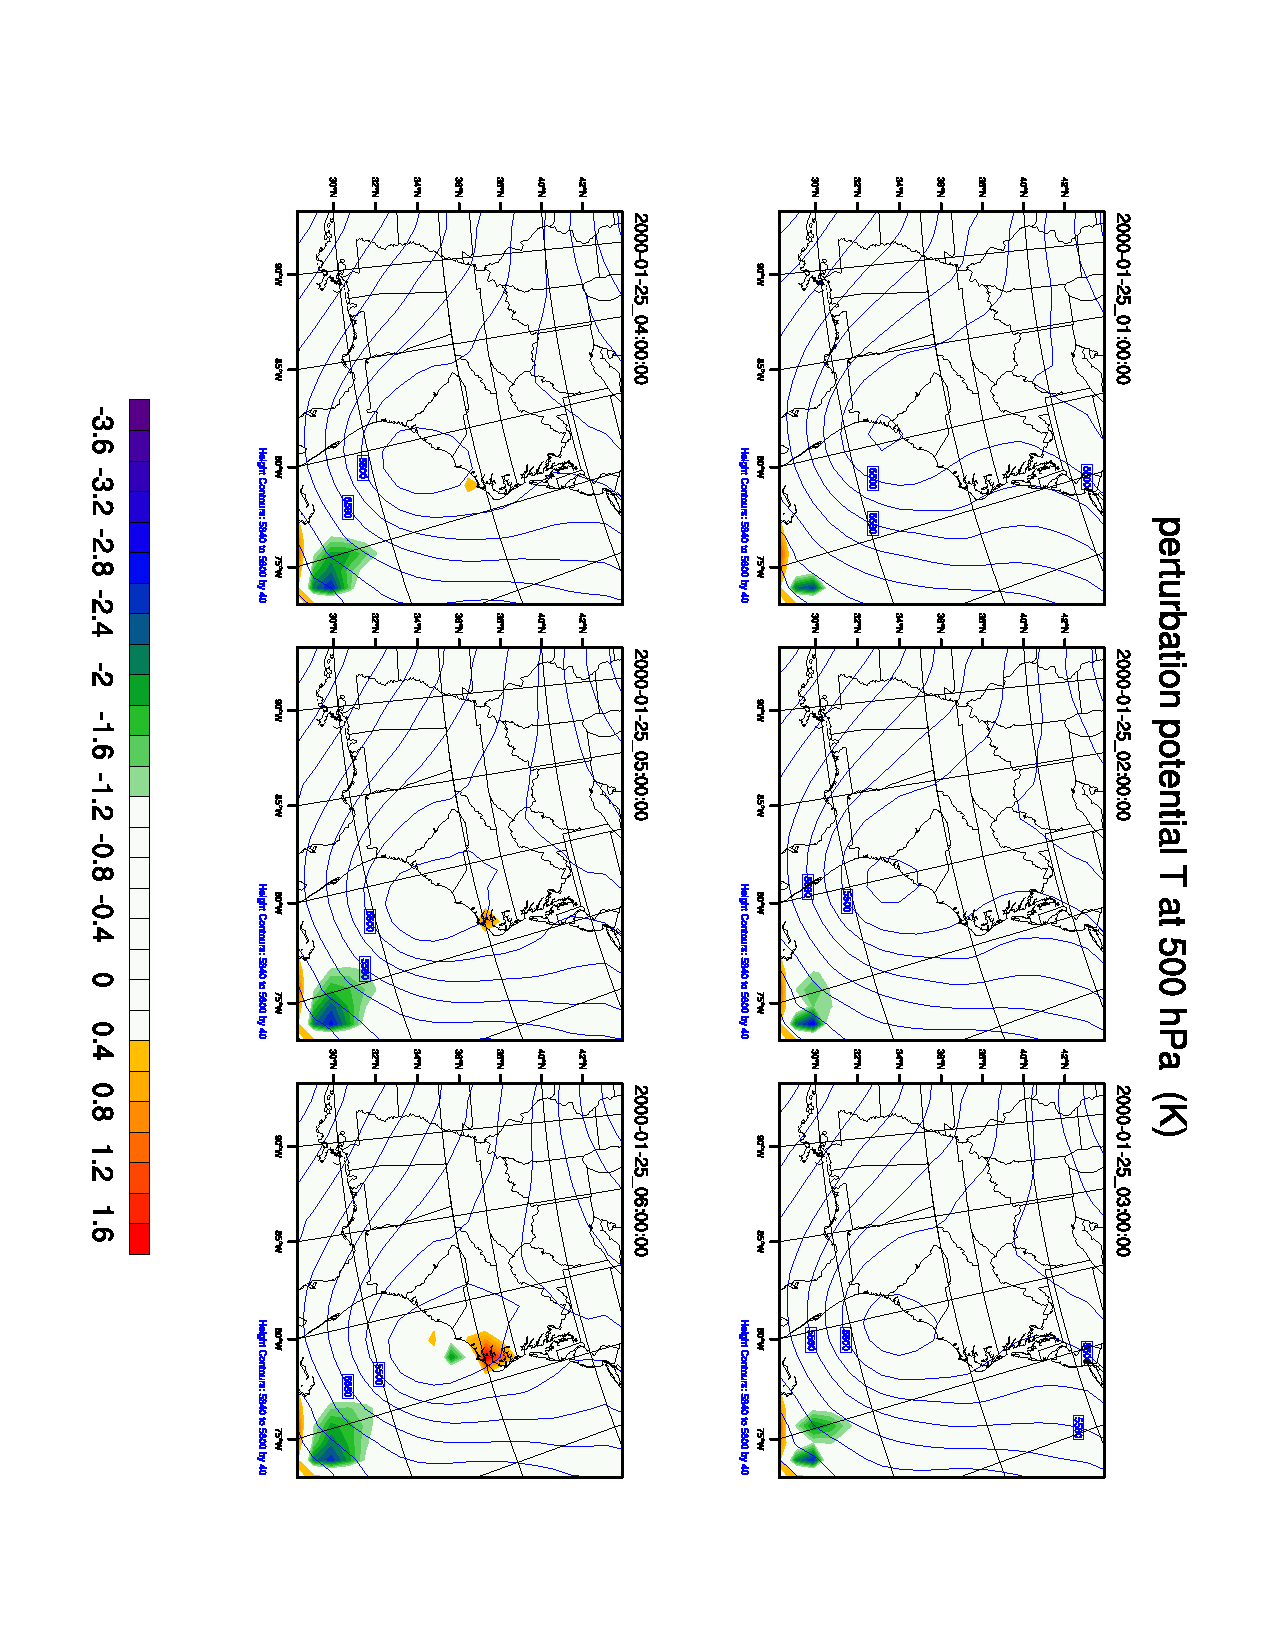
\includegraphics[trim=363 500 66 85, clip=true, angle=90, width=0.7\textwidth]{figures/boundary_6h} 
\end{figure} 
\end{frame}

\begin{frame}
\frametitle{500hPa $\theta$ increments from 0--6 h w/o LBC control}
\begin{figure} 
\centering 
\centering 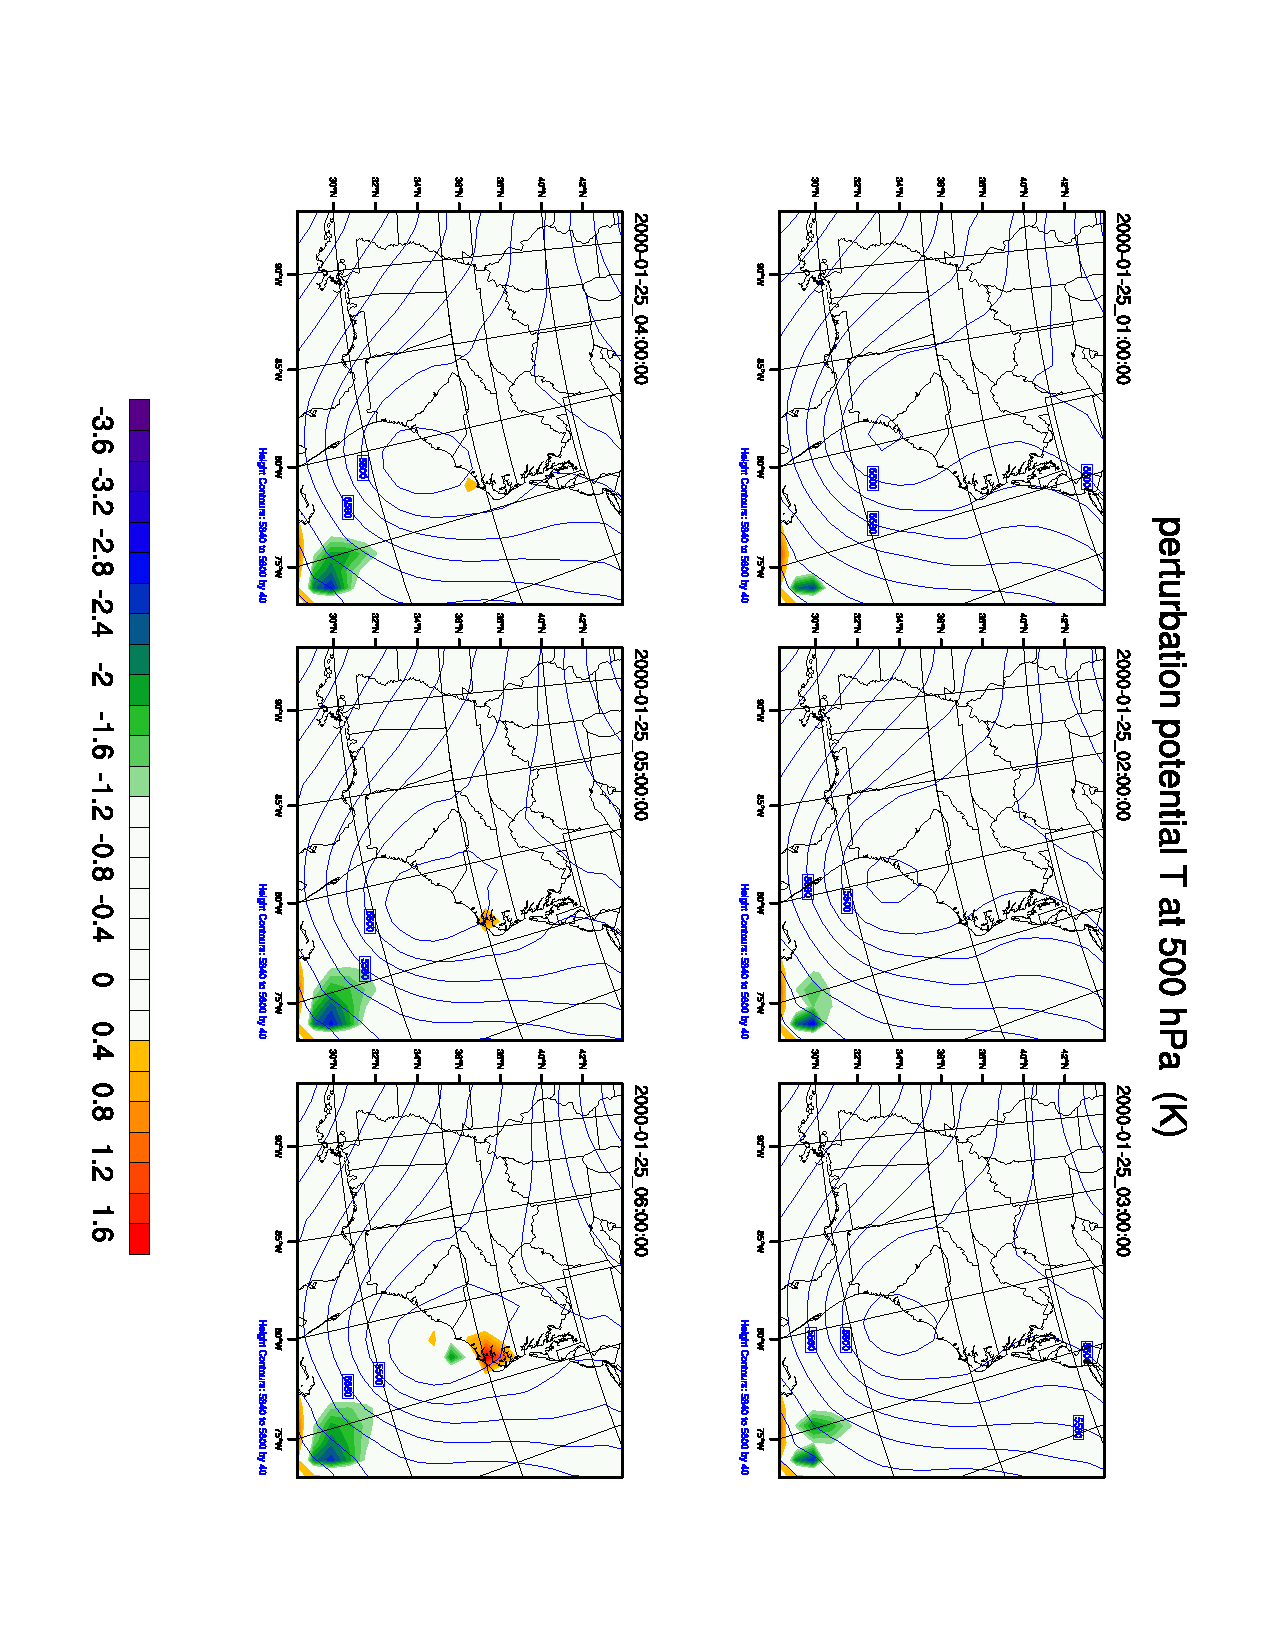
\includegraphics[trim=363 291 66 295, clip=true, angle=90, width=0.7\textwidth]{figures/boundary_6h} 
\end{figure} 
\end{frame}

\begin{frame}
\frametitle{500hPa $\theta$ increments from 0--6 h w/o LBC control}
\begin{figure} 
\centering 
\centering 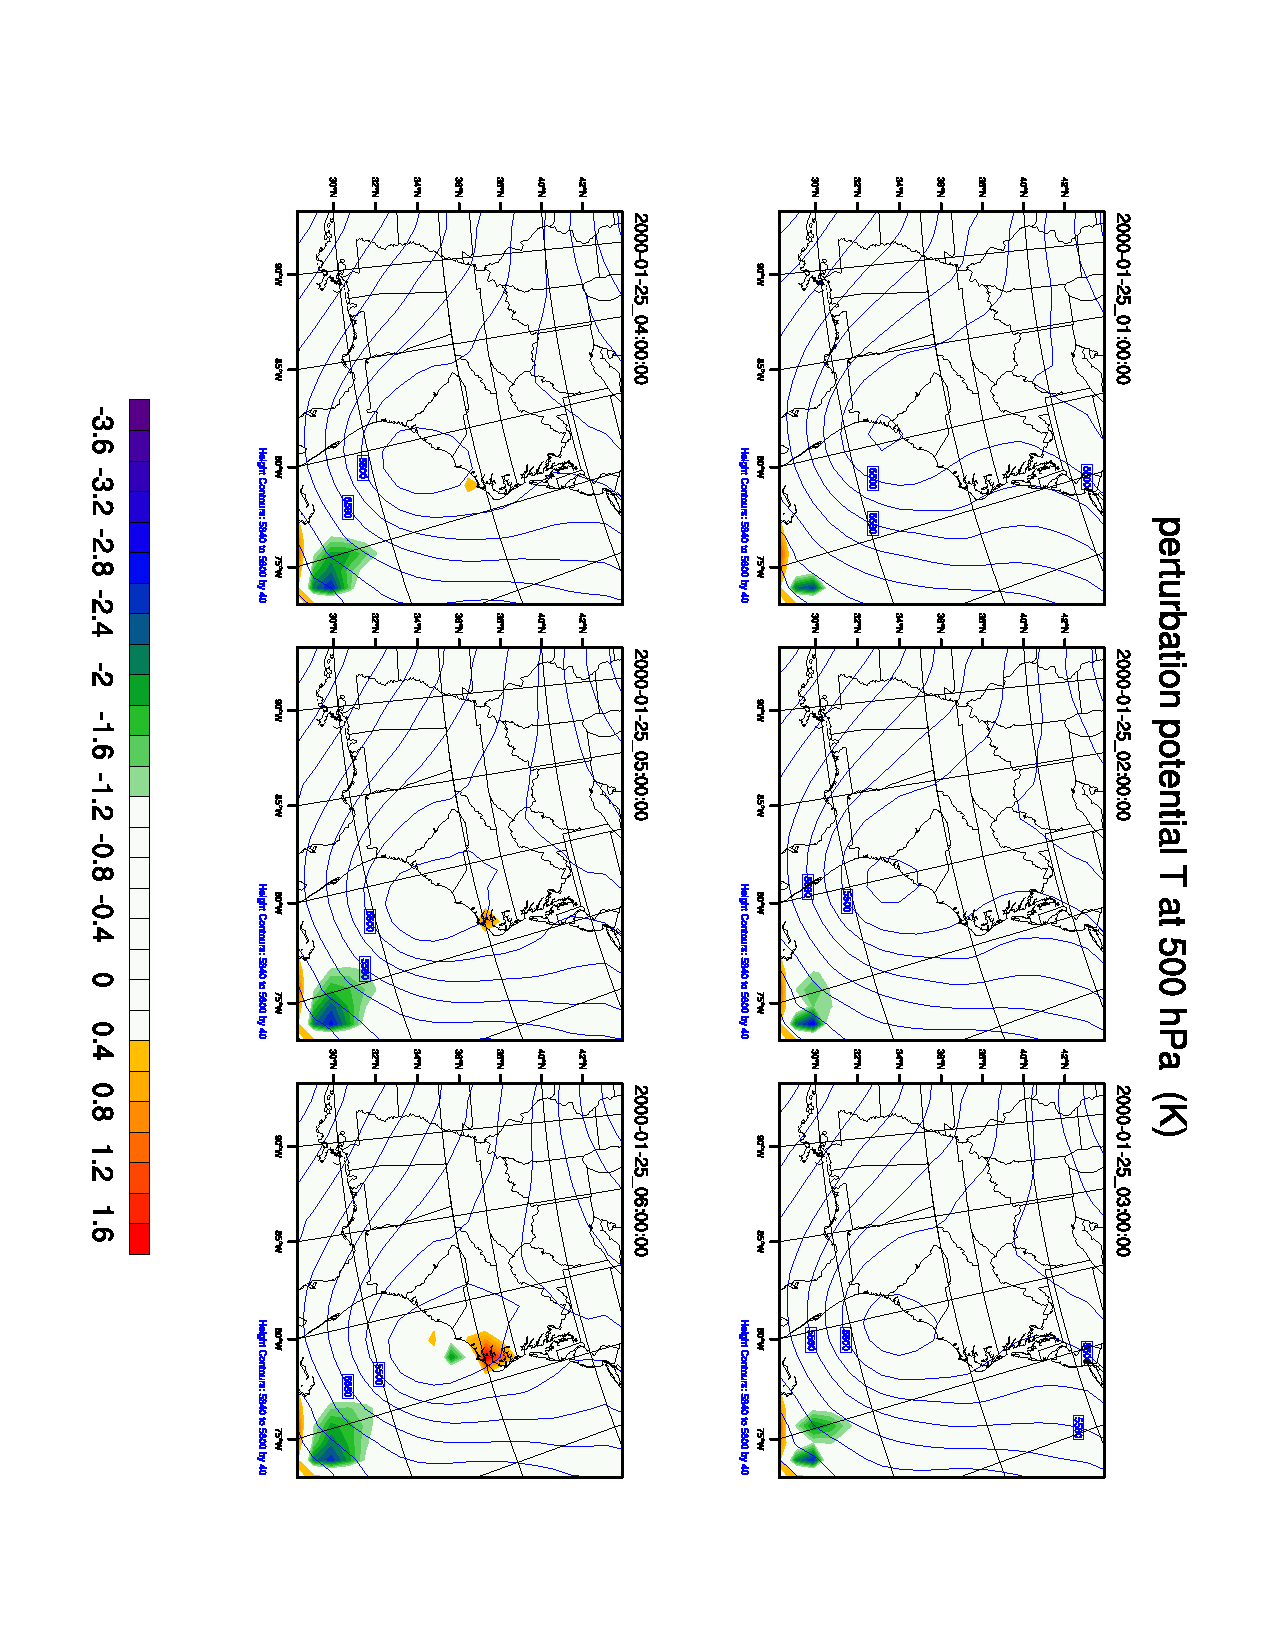
\includegraphics[trim=363 82 66 502, clip=true, angle=90, width=0.7\textwidth]{figures/boundary_6h} 
\end{figure} 
\end{frame}

\begin{frame}
\frametitle{500hPa $\theta$ increments from 0--6 h w/o LBC control}
\begin{figure} 
\centering 
\centering 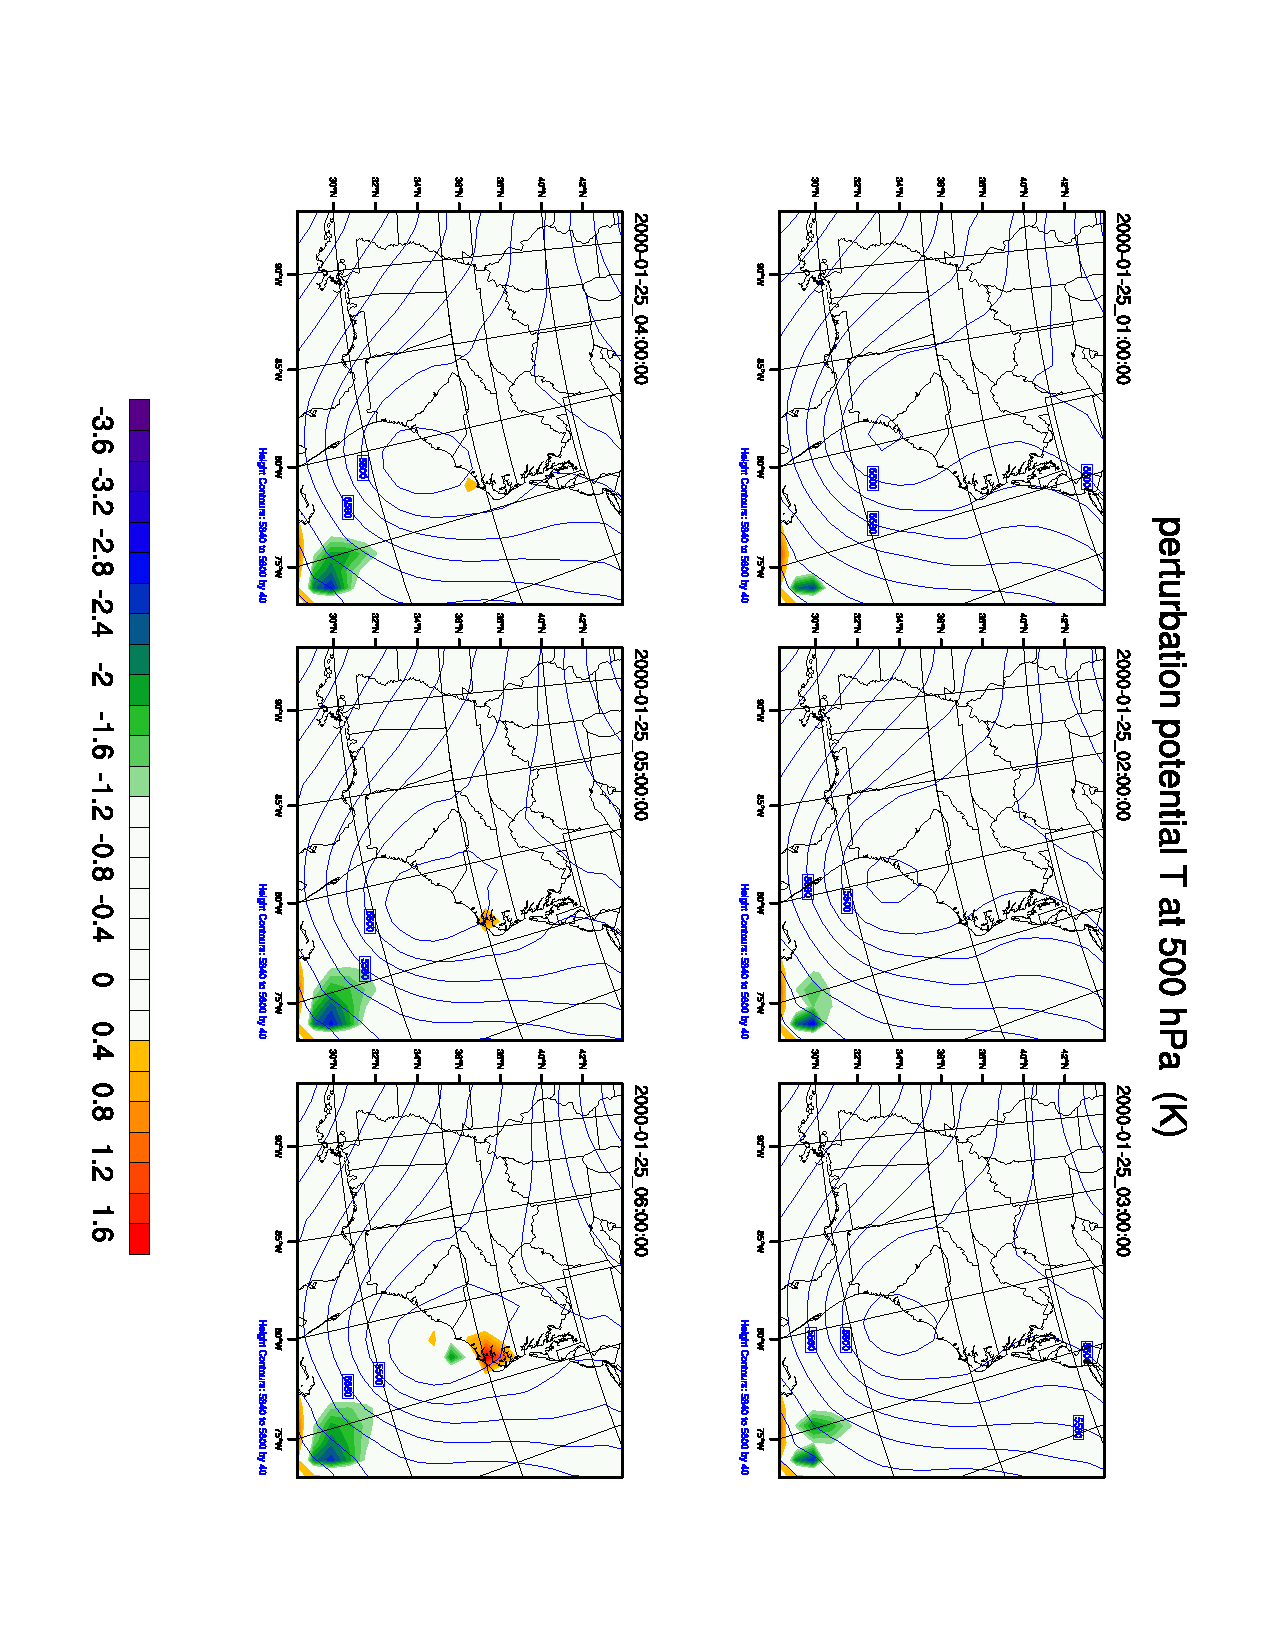
\includegraphics[trim=132 500 300 85, clip=true, angle=90, width=0.7\textwidth]{figures/boundary_6h} 
\end{figure} 
\end{frame}

\begin{frame}
\frametitle{500hPa $\theta$ increments from 0--6 h w/o LBC control}
\begin{figure} 
\centering 
\centering 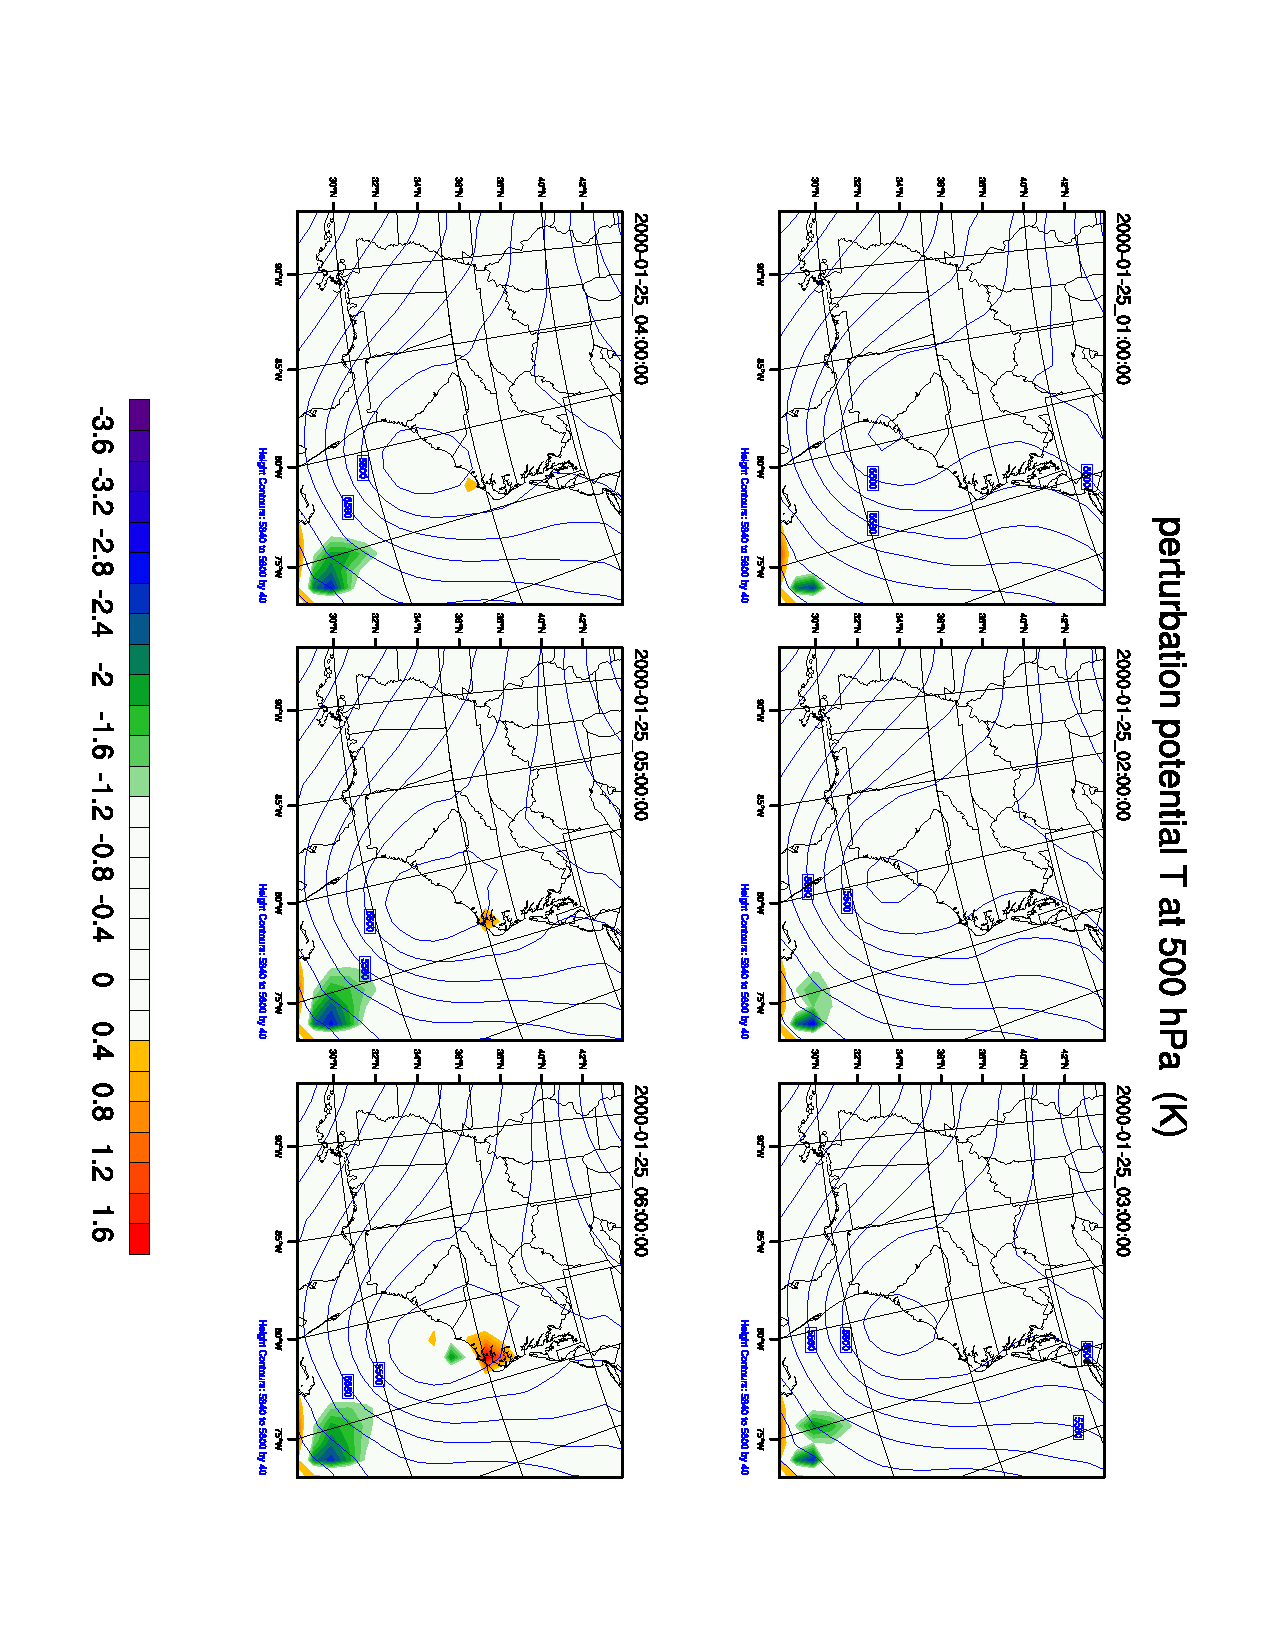
\includegraphics[trim=132 291 300 293, clip=true, angle=90, width=0.7\textwidth]{figures/boundary_6h} 
\end{figure} 
\end{frame}

\begin{frame}
\frametitle{500hPa $\theta$ increments from 0--6 h w/o LBC control}
\begin{figure} 
\centering 
\centering 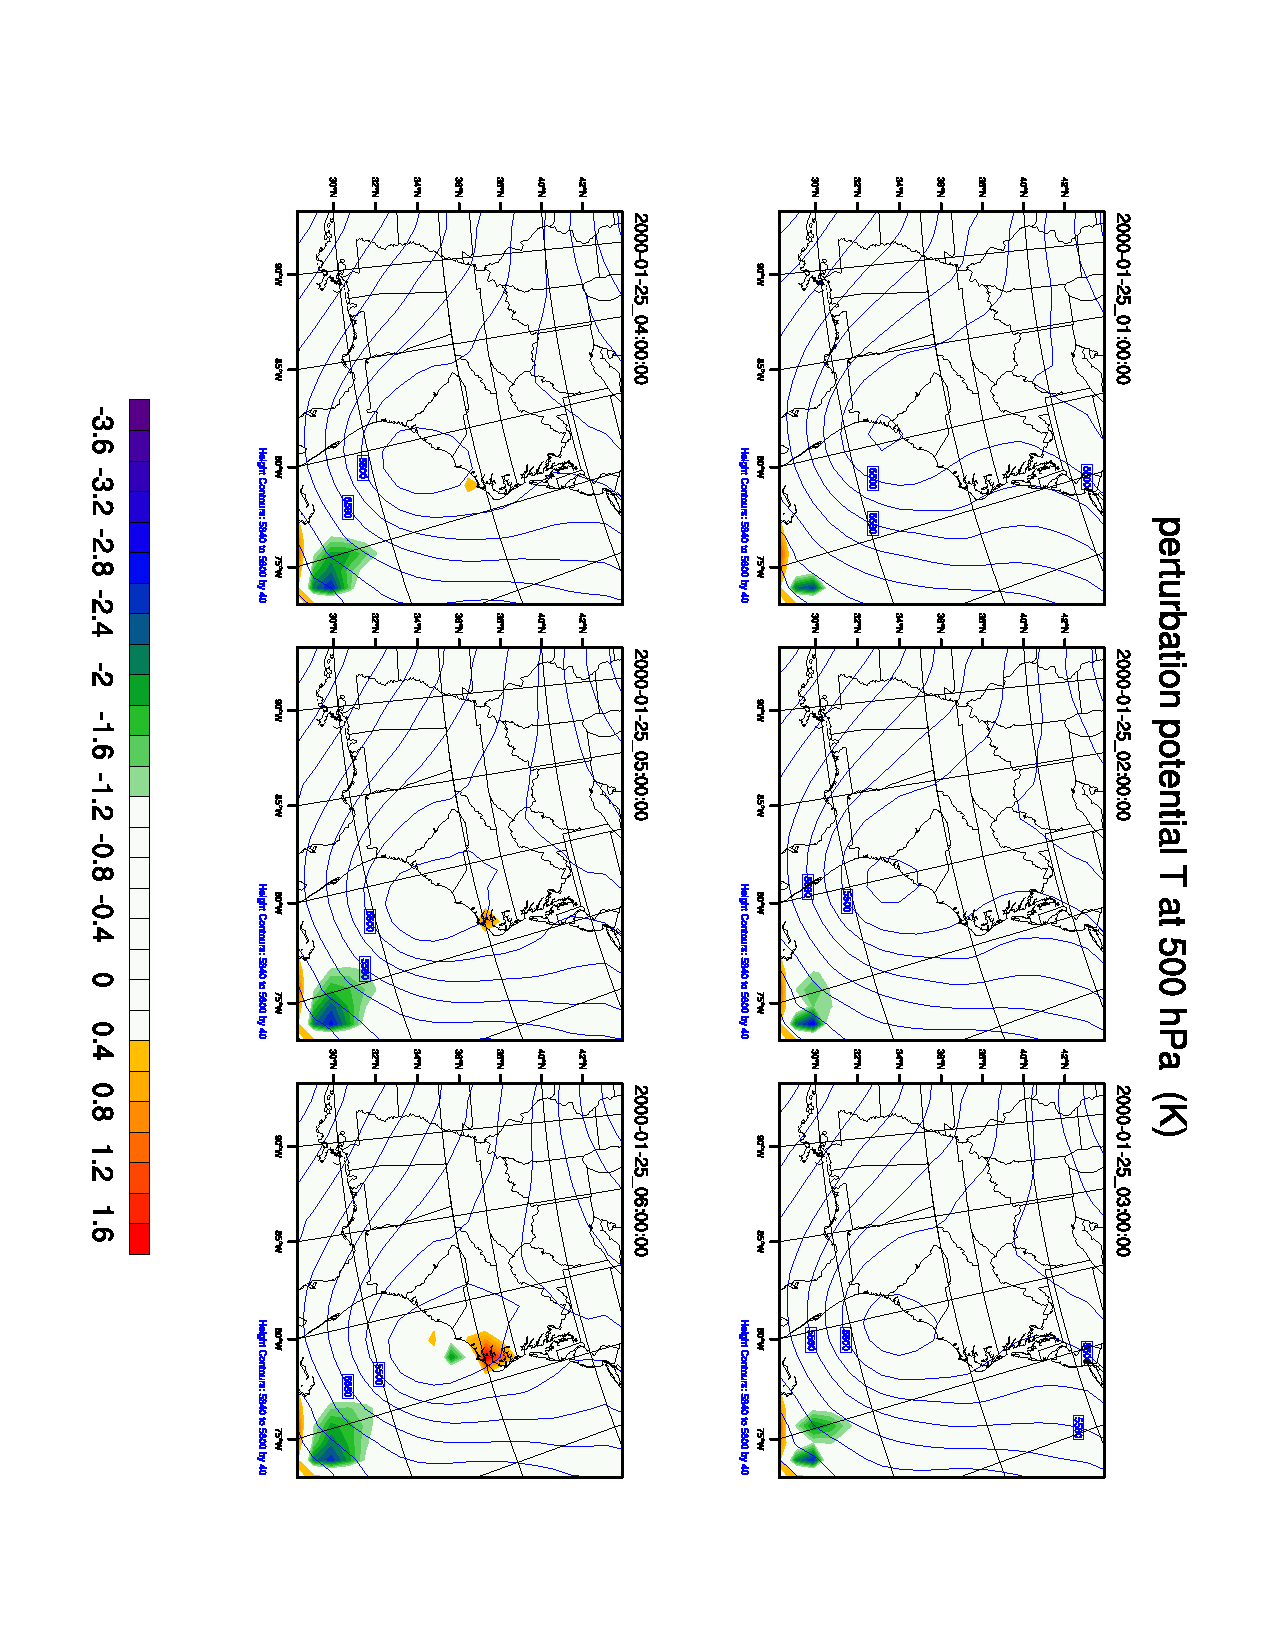
\includegraphics[trim=132 82 300 502, clip=true, angle=90, width=0.7\textwidth]{figures/boundary_6h} 
\end{figure} 
\end{frame}

%\begin{frame}
%\frametitle{500hPa $\theta$ increments from 0--6 h with LBC control}
%\begin{figure} 
%\centering 
%\begin{minipage}[c]{0.3\linewidth} 
%\centering 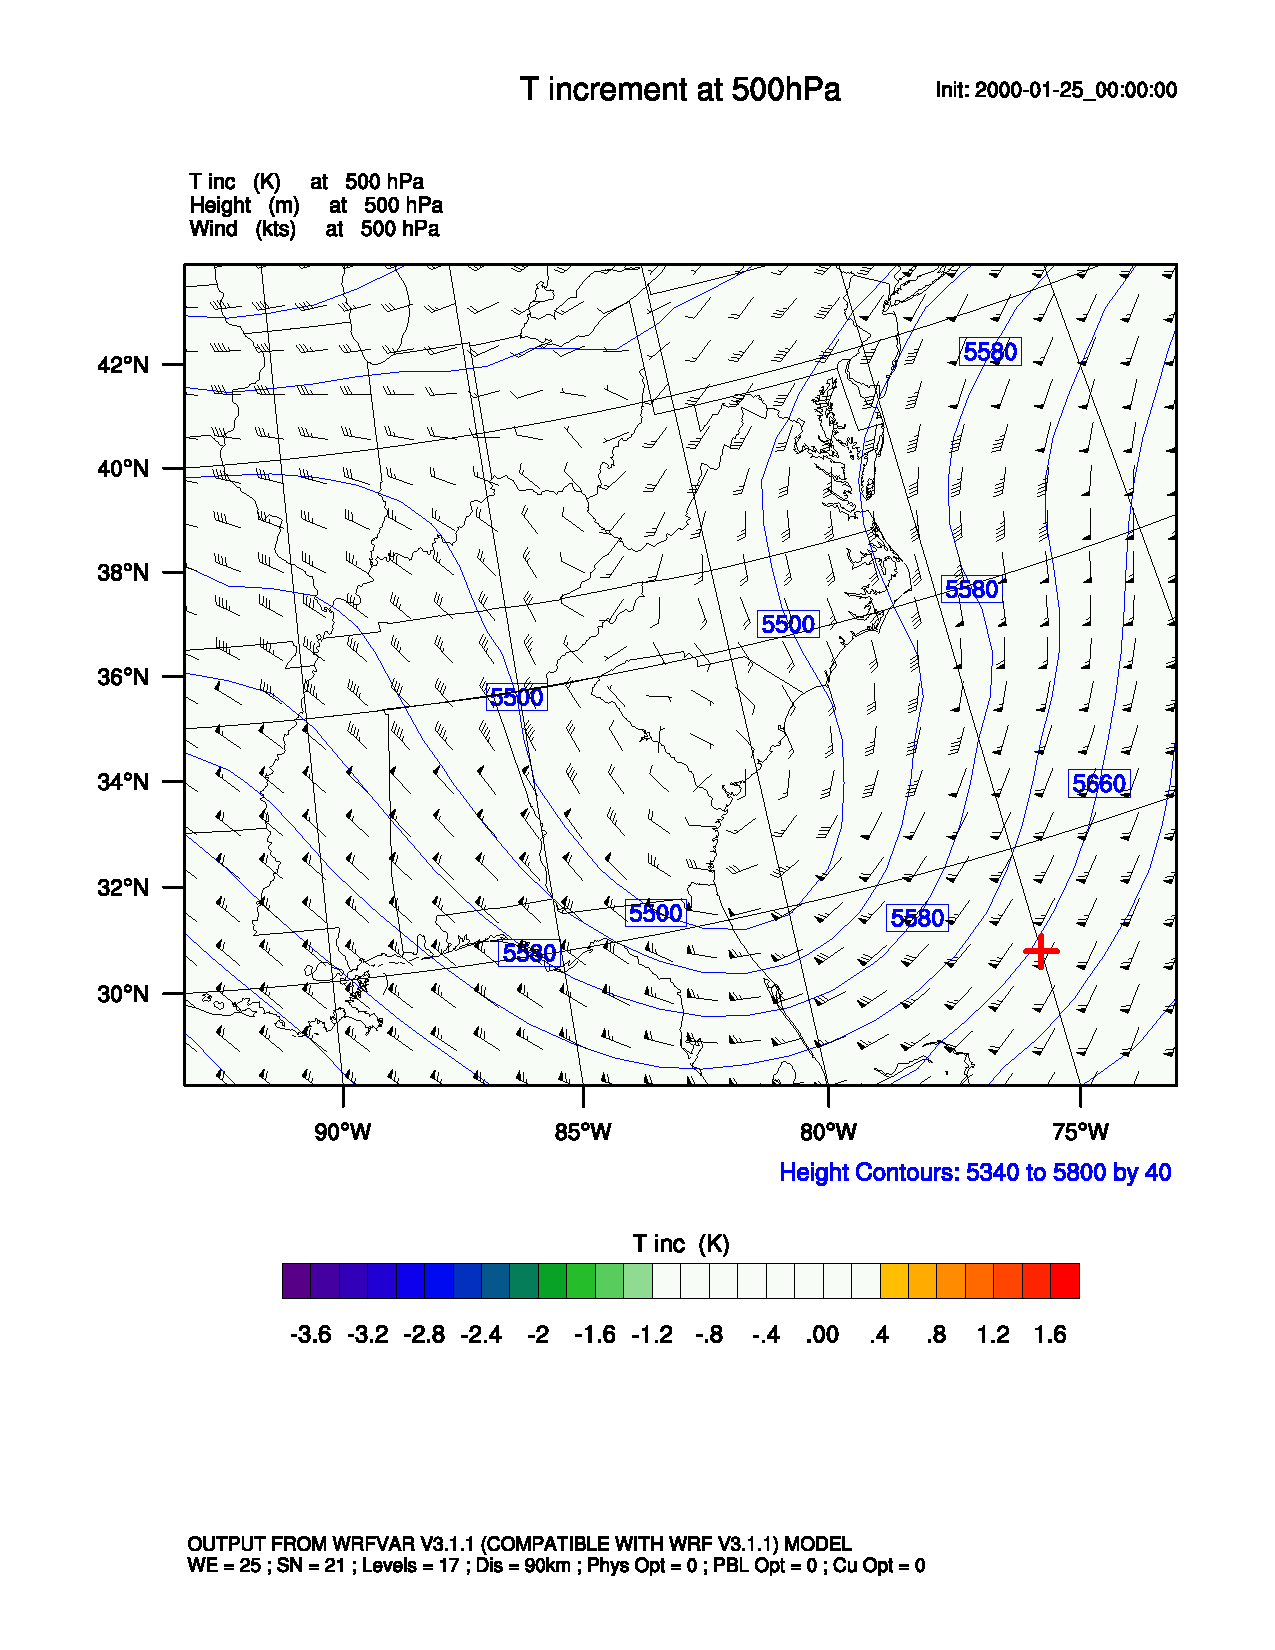
\includegraphics[trim=0 220 0 110, clip=true, width=1.0\textwidth]{figures/boundary_lbc} 
%\end{minipage}% 
%\begin{minipage}[c]{0.8\linewidth} 
%\centering \includegraphics[trim=100 0 60 0, clip=true, angle=90, width=1.0\textwidth]{figures/boundary_lbc_6h} 
%\end{minipage} 
%\end{figure} 
%\end{frame}

\begin{frame}
\frametitle{500hPa $\theta$ increments from 0--6 h with LBC control}
\begin{figure} 
\centering 
\centering 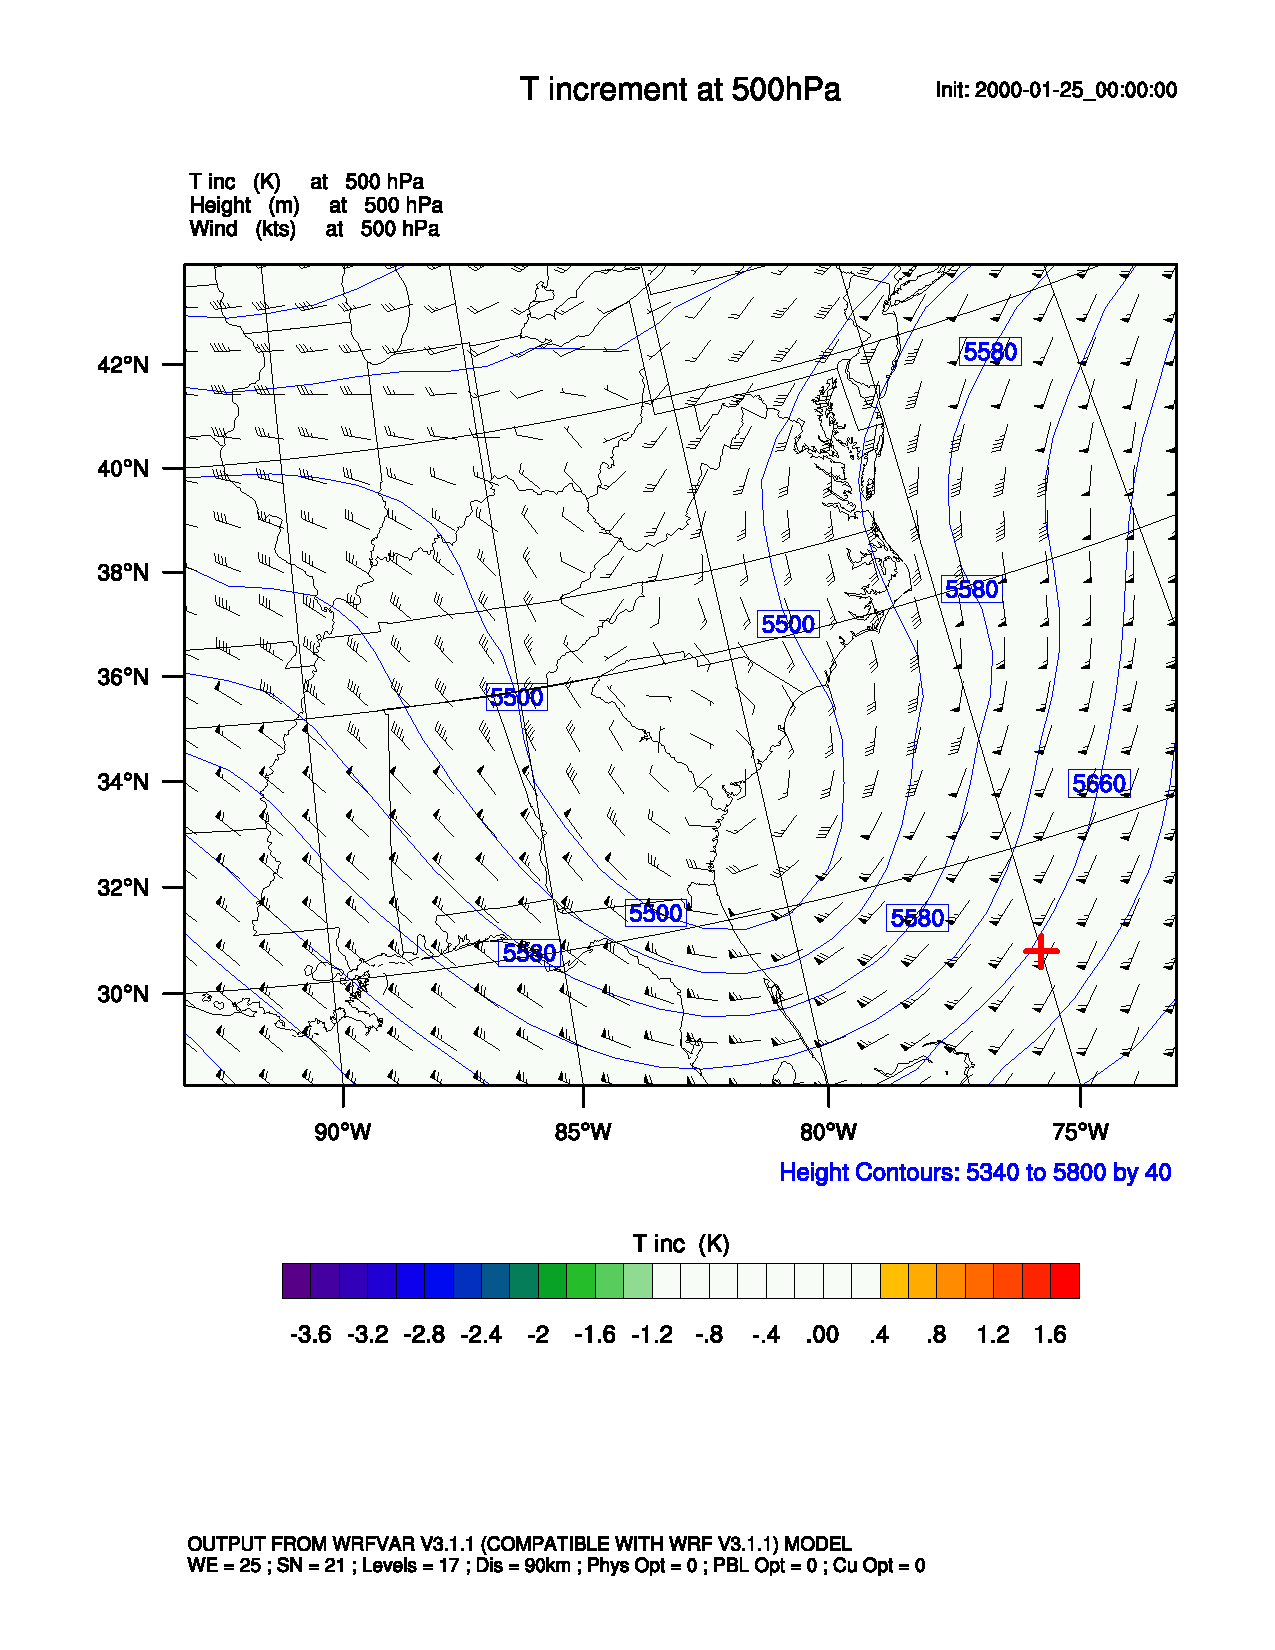
\includegraphics[trim=40 230 40 110, clip=true, width=0.7\textwidth]{figures/boundary_lbc} 
\end{figure} 
\end{frame}

\begin{frame}
\frametitle{500hPa $\theta$ increments from 0--6 h with LBC control}
\begin{figure} 
\centering 
\centering \includegraphics[trim=363 500 66 85, clip=true, angle=90, width=0.7\textwidth]{figures/boundary_lbc_6h} 
\end{figure} 
\end{frame}

\begin{frame}
\frametitle{500hPa $\theta$ increments from 0--6 h with LBC control}
\begin{figure} 
\centering 
\centering \includegraphics[trim=363 291 66 295, clip=true, angle=90, width=0.7\textwidth]{figures/boundary_lbc_6h} 
\end{figure} 
\end{frame}

\begin{frame}
\frametitle{500hPa $\theta$ increments from 0--6 h with LBC control}
\begin{figure} 
\centering 
\centering \includegraphics[trim=363 82 66 502, clip=true, angle=90, width=0.7\textwidth]{figures/boundary_lbc_6h} 
\end{figure} 
\end{frame}

\begin{frame}
\frametitle{500hPa $\theta$ increments from 0--6 h with LBC control}
\begin{figure} 
\centering 
\centering \includegraphics[trim=132 500 300 85, clip=true, angle=90, width=0.7\textwidth]{figures/boundary_lbc_6h} 
\end{figure} 
\end{frame}

\begin{frame}
\frametitle{500hPa $\theta$ increments from 0--6 h with LBC control}
\begin{figure} 
\centering 
\centering \includegraphics[trim=132 291 300 293, clip=true, angle=90, width=0.7\textwidth]{figures/boundary_lbc_6h} 
\end{figure} 
\end{frame}

\begin{frame}
\frametitle{500hPa $\theta$ increments from 0--6 h with LBC control}
\begin{figure} 
\centering 
\centering \includegraphics[trim=132 82 300 502, clip=true, angle=90, width=0.7\textwidth]{figures/boundary_lbc_6h} 
\end{figure} 
\end{frame}

\begin{frame}
\frametitle{Remark}
\begin{itemize}
\item The Final $J_{lbc}$ is increased from 0 to 0.5 ( 0 to 0.01 w/o LBC control) \pause
\item LBC control has significant impact on the initial potential temperature perturbation \pause
\item Under the flow dependent context, the response in IC to the 6h observation should be outside the domain. If the LBC play a role in the minimization, the main analysis response should be in LBC, otherwise, some fake or overestimated responses will be appeared in IC along the south boundary \pause
\item For 0--6h perturbation evolution, there is perturbation entering into the south boundary with LBC control, and the location of the 6h perturbation is much better than that w/o LBC control
\end{itemize}
\end{frame}

\section{Summary}

\begin{frame}
\frametitle{Summary and Vision}
\begin{itemize}
\item Single observation experiments confirm the preliminary implementation of  LBC control in WRF 4D-Var \pause
\item Inclusion of LBC control in 4D-Var helps to obtain a analysis which fits observation better (not shown here) \pause
\item Preliminary real observation experiments with LBC control don't show noticeable improvement \pause
\item Deliberated experiments should be designed to evaluate the impact of LBC control in real case \pause
\item More efforts are needed \ldots{}
\end{itemize}
\end{frame}

\end{document}
